
% This include all the settings that we should use for the document
\newcommand{\PDFTitle}{Using the DESim Application \\ with\hdlAdj~\hdlName~Designs}
\newcommand{\commonPath}{../../../Tutorials/Common}
\input{\commonPath/Docs/defaulttext.tex}
\input{\commonPath/Docs/preamble.tex}

%%%%%%%%%%%%%%%%%%%%%%%%%
% Add title
\newcommand{\doctitle}{Using the DESim Application \\ with\hdlAdj\hdlName~Designs}
\newcommand{\dochead}{Using the DESim Application}
% Usually no need to change these two lines
\title{\fontfamily{phv}\selectfont{\doctitle} }
\chead{ \small{\textsc{\bfseries \dochead} } }
% Customizations
\newenvironment{ctabbing}%
{\begin{center}\begin{minipage}{\textwidth}\begin{tabbing}}
{\end{tabbing}\end{minipage}\end{center}}

%%%%%%%%%%%%%%%%%%%%%%%%%
% Allows multiple figures per page

\renewcommand\floatpagefraction{.9}
\renewcommand\topfraction{.9}
\renewcommand\bottomfraction{.9}
\renewcommand\textfraction{.1}   
\setcounter{totalnumber}{50}
\setcounter{topnumber}{50}
\setcounter{bottomnumber}{50}
\raggedbottom

\definecolor{AppleGreen}{rgb}{0.55, 0.71, 0.0}
\newcommand{\green}[1]{{\color{AppleGreen}\sf{#1}}}

\renewcommand{\versnum}{~} %version number quartus/AMP
\newif\ifquesta
\questatrue % comment out to not include Questa
\newif\iflinux
%\linuxtrue % comment out to not include Linux

%%%%%%%%%%%%%%%%%%
%%% DOCUMENT START
\begin{document}
\begin{table}
    \centering
    \begin{tabular}{p{5cm}p{4cm}}
        \hspace{-3cm}
        &
        \raisebox{1\height}{\parbox[h]{0.5\textwidth}{\Large\fontfamily{phv}\selectfont{\textsf{\doctitle}}}}
    \end{tabular}
    \label{tab:logo}
\end{table}

\colorbox[rgb]{0,0.384,0.816}{\parbox[h]{\textwidth}{\color{white}\textsf{\textit{\textBar}}}}

\thispagestyle{plain}
 
\section{Introduction}

This tutorial introduces the {\it DESim}\textsuperscript{\textregistered} application, 
which you can use to {\it simulate} the implementation of circuits that are specified 
with \hdlName~code\ifnotSV{}\else{, including System Verilog extensions}\fi, 
in an Altera\textsuperscript{\textregistered} FPGA device. 
The {\it DESim} application provides a {\it graphical user interface} 
(GUI) that represents some of the features of a {\it DE1-SoC} (or similar) FPGA board, 
as described in the \texttt{Teaching and Projects Boards} section of the 
{\small \href{https://www.fpgacademy.org/boards.html} {FPGAcademy.org}} website.
The {\it DESim} application serves as a ``front end'' for 
\ifquesta {either the {\it ModelSim} or {\it Questa}}
\else {the {\it ModelSim}} \fi
Simulator. Using the {\it DESim} GUI you can compile your
\hdlName~code and then run the Simulator. Its inputs are provided by 
clicking on features in the {\it DESim} GUI, which also shows results produced by 
the Simulator on displays that look like the ones on a {\it DE1-SoC} board.

{\bf Contents:}
\vspace{-1em}
\begin{itemize}
\item Getting started with the {\it DESim} application
\item Compiling and simulating {\it DESim} sample projects
\item Simulating a circuit that includes a memory module
\item Making your own {\it DESim} project
\item Troubleshooting problems with the {\it DESim} application
\end{itemize}

{\bf Requirements:}
\vspace{-1em}
\begin{itemize}
	\item A good working knowledge of the \hdlName~hardware description 
    language\ifnotSV{}\else{, including some of its basic System Verilog extensions}\fi
\item A computer running Microsoft\textsuperscript{\textregistered}
Windows\textsuperscript{\textregistered} (version 10 or 11 is
recommended)\iflinux{ or Ubuntu Linux}\fi
\item The {\it DESim} application: an {\it Installation Guide} 
is available in the \texttt{Software} tab on 
\href{https://www.fpgacademy.org/tools.html}{FPGAcademy.org}.
\item 
\ifquesta
{{\it ModelSim-Intel FPGA} software or {\it Questa-Intel FPGA} software: instructions for 
obtaining these Simulators are included in the {\it DESim Installation Guide}. {\it DESim} can 
be used with the {\it ModelSim} releases that are part of versions 18.1 to 20.1 of the 
Altera {\it Quartus Prime} CAD system, or any release of {\it Questa} that is provided as
part of {\it Quartus Prime}.} We recommend using {\it ModelSim}, because it does not require a
license, whereas {\it Questa} has a licensing requirement.
\else
{{\it ModelSim-Intel FPGA} software: instructions for obtaining the {\it ModelSim}
Simulator are included in the {\it DESim Installation Guide}. {\it DESim} can be used with 
the {\it ModelSim} releases that are part of the Altera {\it Quartus Prime} CAD system, 
versions 18.1 to 20.1.}
\fi
\item You should know how to simulate \hdlName~code using a {\it testbench}, as described
in the tutorial\ifquesta{s}\fi
{\it~Using ModelSim with Testbenches}\ifquesta{~and {\it Using Questa with
Testbenches}}\fi. \ifquesta{These tutorials are}\else{This tutorial is}\fi~available in 
the \texttt{Tutorials} tab on
\href{https://www.fpgacademy.org/tutorials.html}{FPGAcademy.org}.
\end{itemize}

\newpage

\section{Getting Started}
\label{sec:getting_started}
Start the {\it DESim} program by executing the {\it batch} script named {\it DESim\_run.bat},
which is provided in the folder where the {\it DESim} application is installed on your computer. 
You should see the {\it DESim} graphical user interface (GUI), as displayed in 
Figure~\ref{fig:gui}, along with the message ``\green{The server is running...}'' at 
the top of the {\it message pane} in the GUI. If you do not see this message, but instead 
see a message \red{Server setup failed...}, then the {\it DESim} software is not working
properly and should be closed. In this case, refer to the troubleshooting guide that is
provided in Section \ref{sec:trouble}.

On the right-hand side of Figure~\ref{fig:gui}, the \texttt{LEDs} represent the 
red lights \red{LEDR$_{9-0}$} that are provided on a DE1-SoC (or similar)
FPGA board.  The \texttt{Switches} correspond to the board's \blue{SW$_{9-0}$} 
slide switches, the \texttt{Push Buttons} to \blue{KEY$_{3-0}$}, and the 
\texttt{Seven-segment Displays} to \red{HEX5}, \red{HEX4}, $\ldots$, \red{HEX0}.
There are also some additional features in the GUI called \texttt{PS/2 Keyboard}, 
\texttt{Parallel Ports}, and \texttt{VGA Display}. Each of these features is discussed 
in Section~\ref{sec:advanced}.

\begin{figure}[H]
	\begin{center}
        \setlength{\fboxsep}{0pt}
        \fbox{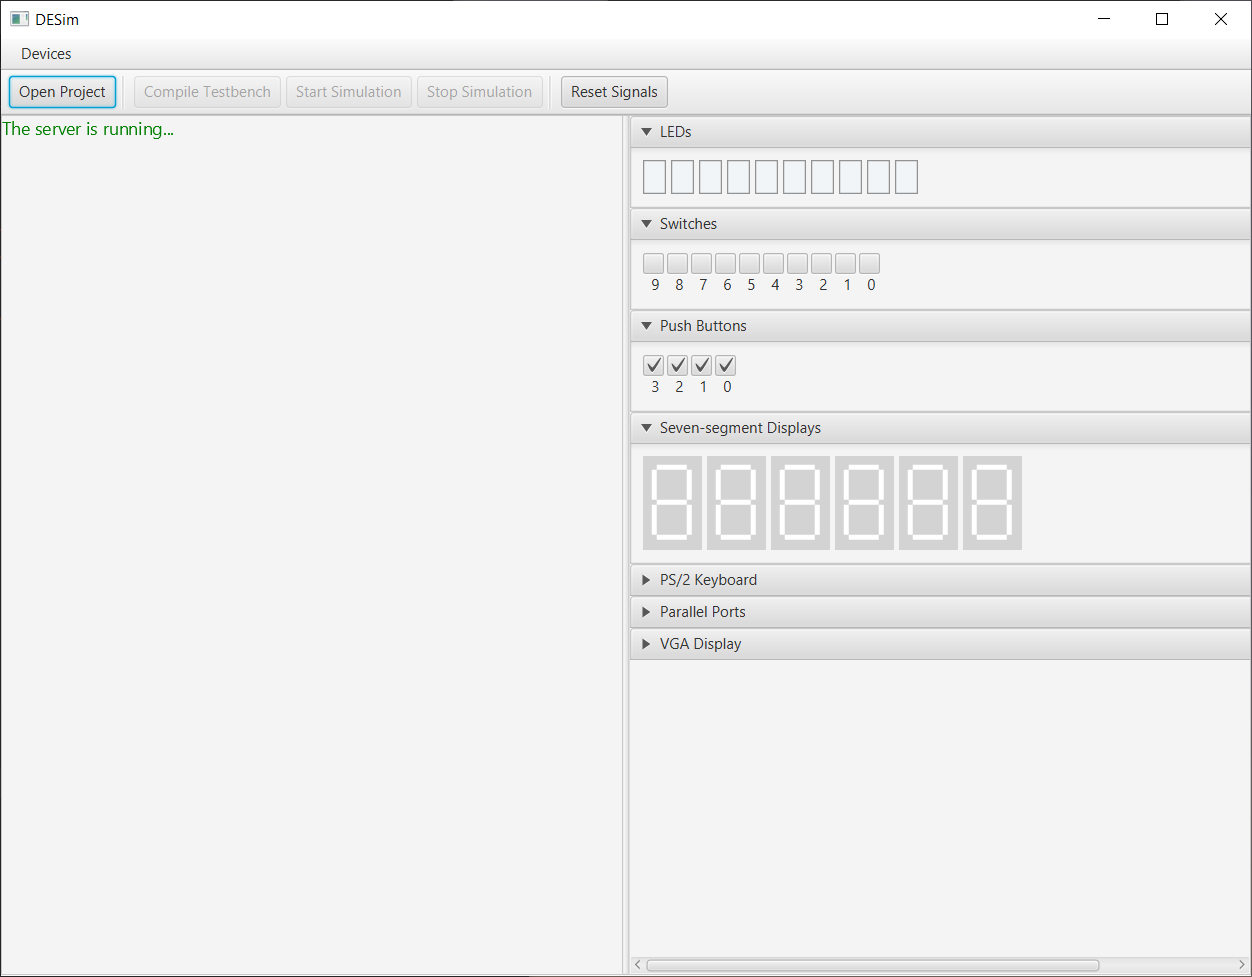
\includegraphics[width = \textwidth]{figures/DESim_GUI.png}}
	\end{center}
		  \caption{The {\it DESim} GUI.}
	\label{fig:gui}
\end{figure}

The {\it DESim} application works in the context of a {\it project}. To introduce the features of 
the {\it DESim} GUI, we will first open an existing project. This example is a multibit 
{\it adder}, which is provided as a {\it sample} project that is installed along with the 
{\it DESim} software. Referring to Figure~\ref{fig:gui}, click on the \texttt{Open Project} button 
to reach the dialogue displayed in Figure~\ref{fig:open_windows}. As indicated in the figure, 
navigate to the {\it DESim} \texttt{demos/\demos} folder, click on the \texttt{adder} folder, and
then click on the \texttt{Select Folder} button to open the project. In the DESim GUI you
should now see the message ``\green{Project `adder' opened.}''.

\begin{figure}[h]
	\begin{center}
        \setlength{\fboxsep}{0pt}
        \ifverilog 
            \ifnotSV
                \fbox{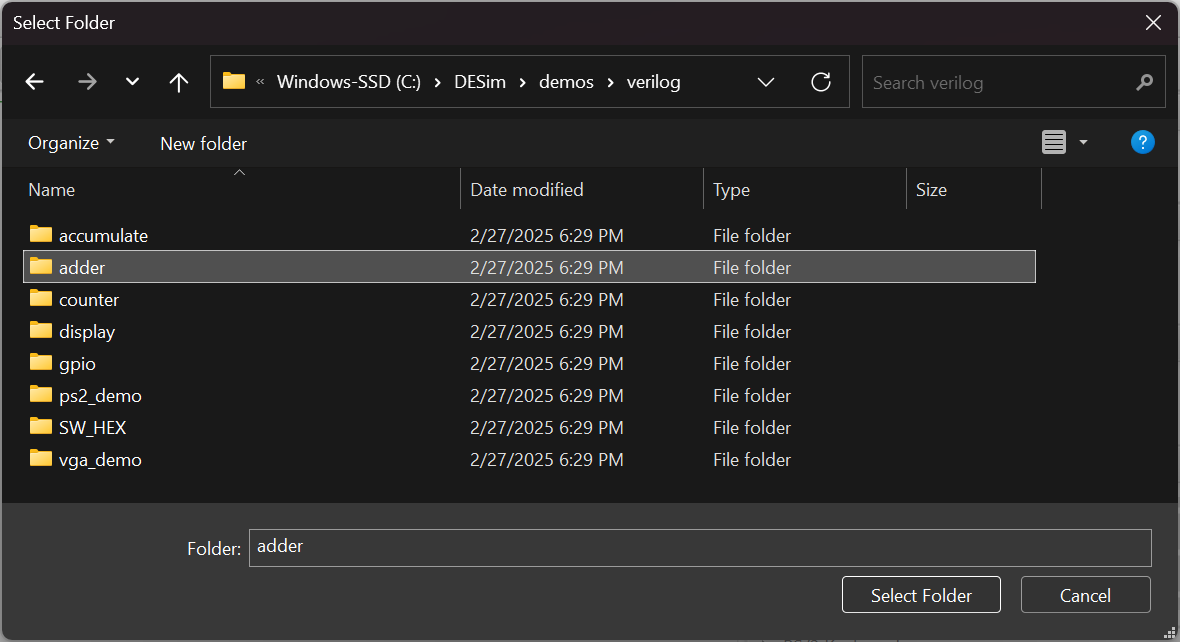
\includegraphics[scale=0.5]{figures/open_adder_windows.png}}
            \else
                \fbox{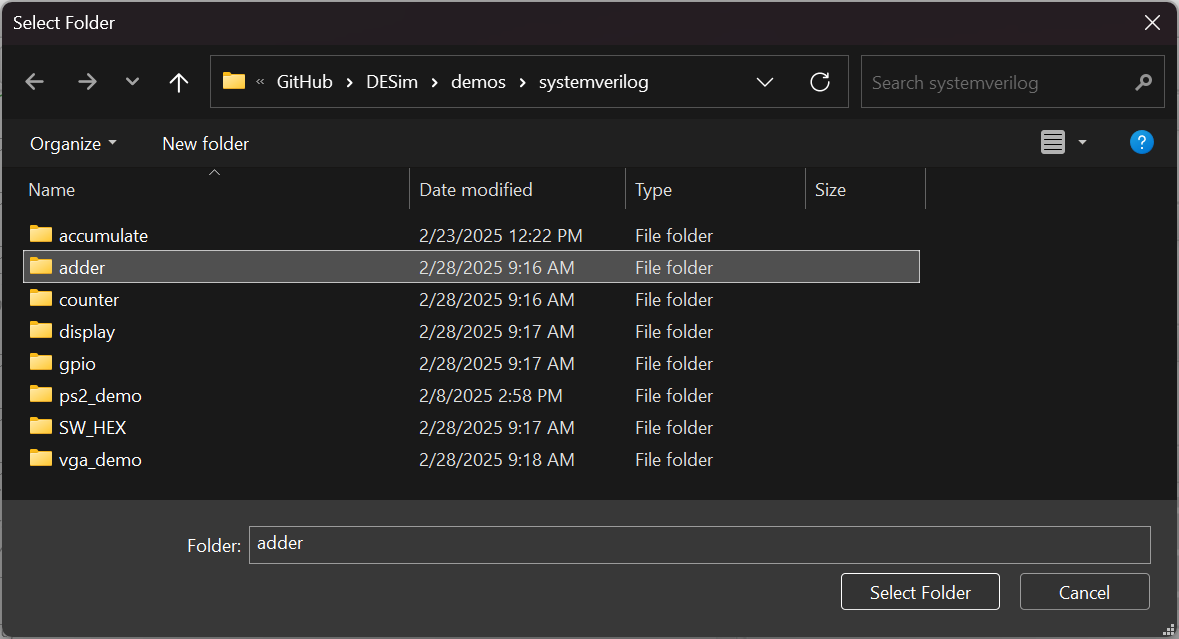
\includegraphics[scale=0.5]{figures/open_adder_sv_windows.png}}
            \fi
        \else 
            \fbox{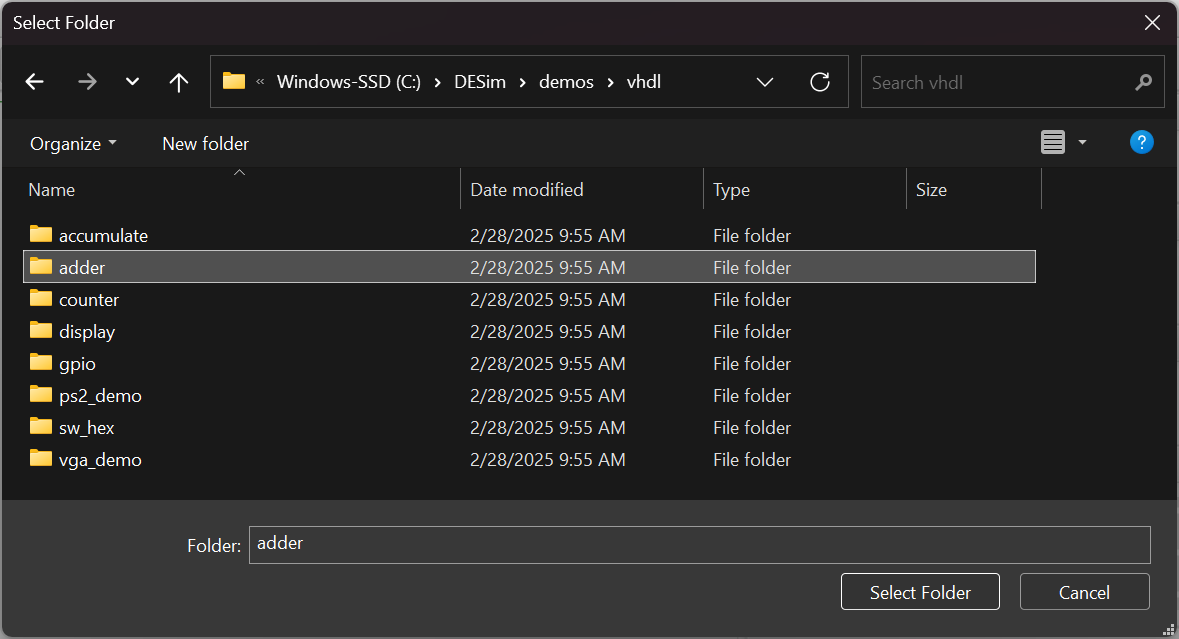
\includegraphics[scale=0.5]{figures/open_adder_vhdl_windows.png}}
        \fi
	\end{center}
		  \caption{Opening the {\it adder} project.}
	\label{fig:open_windows}
\end{figure}

All DESim projects have a similar organization of files and folders, which we can illustrate
by examining the {\it adder} project. Open the {\it File Explorer} (or similar) application in 
Windows and navigate to the filesystem folder named \texttt{demos/\demos/adder}, as depicted in 
Figure~\ref{fig:adder_files}. It contains the folders named \texttt{sim} and \texttt{tb}, 
as well as the files called {\it adder.\hdlFileExt} and {\it top.\hdlFileExt}. There is also 
a {\it Readme.txt} file, which gives a brief description of the usage of the {\it adder} project.

\begin{figure}[h]
	\begin{center}
        \setlength{\fboxsep}{0pt}
        \ifverilog
            \ifnotSV
                \fbox{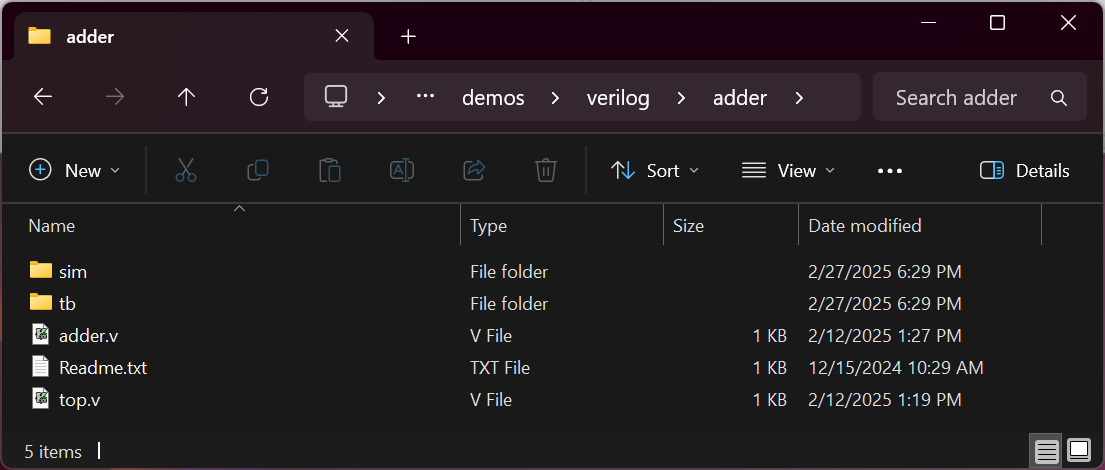
\includegraphics[scale=0.5]{figures/adder_files.png}}
            \else
                \fbox{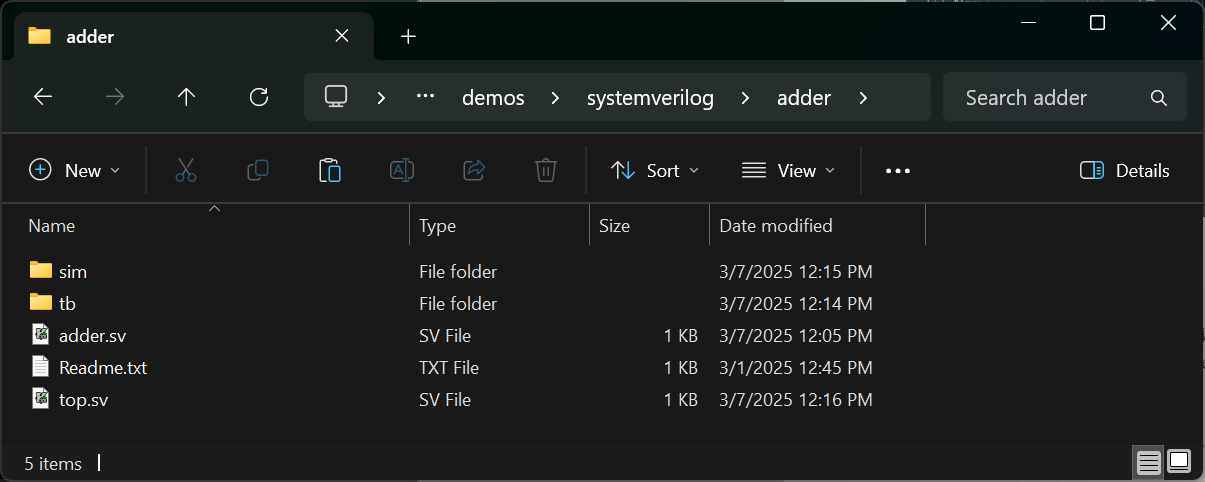
\includegraphics[scale=0.5]{figures/adder_files_sv.png}}
            \fi
        \else
            \fbox{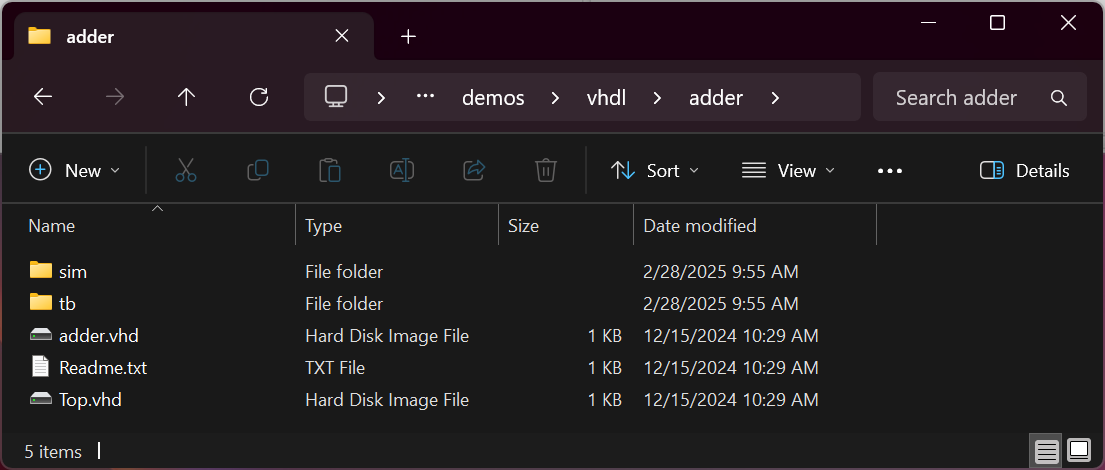
\includegraphics[scale=0.75]{figures/adder_files_vhdl.png}}
        \fi
	\end{center}
		  \caption{Contents of the {\it adder} project.}
	\label{fig:adder_files}
\end{figure}


The {\it adder.\hdlFileExt} file, shown in Figure~\ref{fig:addern}, gives the \hdlName~code
for the adder \hdlModuleName.  We will use the {\it DESim} GUI to specify signal 
values for the adder's inputs, {\it Cin}, {\it X}, and {\it Y}, and then display the
simulation results produced for the outputs, {\it S} and {\it Cout}, on the \texttt{LEDs}. 
To make connections between the adder's ports and the signals that are associated with the
{\it DESim} GUI, we {\it instantiate} the {\it adder} in another \hdlName~\hdlModuleName,
named {\it top}. This \hdlModuleName~is defined in the file {\it top.\hdlFileExt}, which
is displayed in Figure~\ref{fig:top}. Its ports use the signal names that are appropriate for a
top-level \hdlName~\hdlModuleName~which is intended to be implemented on a DE1-SoC board.
For this project the top-level port names are \texttt{SW} and  \texttt{LEDR}.

In {\it top.\hdlFileExt} the {\it adder} \hdlModuleName~is instantiated by the statement
\ifverilog
    \ifnotSV
        \lstinputlisting[language=Verilog,numbers=none,firstline=11,lastline=11]{../../demos/\demos/adder/top.\hdlFileExt}
    \else
        \lstinputlisting[language=Verilog,numbers=none,firstline=11,lastline=11]{../../demos/\demos/adder/top.\hdlFileExt}
    \fi
\else
    \lstinputlisting[language=VHDL,numbers=none,firstline=26,lastline=27]{../../demos/\demos/adder/top.vhd}
\fi

This statement connects the switch {\it SW}$_9$ to the adder's carry-in, {\it Cin}, 
and it connects {\it SW}$_{3-0}$ and  {\it SW}$_{7-4}$ to the adder's {\it X} and {\it Y} 
data inputs, respectively.  The sum, {\it S}, output is attached to {\it LEDR}$_{3-0}$, and 
the carry-out, {\it Cout}, is connected to {\it LEDR}$_4$.

\begin{figure}[h]
\begin{center}
\begin{minipage}[h]{15 cm}
    \ifverilog
        \ifnotSV
            \lstinputlisting[language=Verilog,numbers=none,firstline=8]{../../demos/\demos/adder/adder.\hdlFileExt}
        \else
            \lstinputlisting[language=Verilog,numbers=none,firstline=8, morekeywords={logic}]{../../demos/\demos/adder/adder.\hdlFileExt}
        \fi
    \else
        \lstinputlisting[language=VHDL,numbers=none,firstline=9]{../../demos/\demos/adder/adder.vhd}
    \fi
\end{minipage}
	\caption{The \hdlName~source-code file \texttt{adder.\hdlFileExt}.}
	\label{fig:addern}
\end{center}
\end{figure}

\begin{figure}[h]
\begin{center}
\ifverilog
\begin{minipage}[h]{15 cm}
\else
\begin{minipage}[h]{17 cm}
\fi
    \ifverilog
        \ifnotSV
            \lstinputlisting[language=Verilog,numbers=none,firstline=7]{../../demos/\demos/adder/top.\hdlFileExt}
        \else
            \lstinputlisting[language=Verilog,numbers=none,firstline=7, morekeywords={logic}]{../../demos/\demos/adder/top.\hdlFileExt}
        \fi
	\else
        \lstinputlisting[language=VHDL,numbers=none,firstline=8]{../../demos/\demos/adder/top.vhd}
    \fi
	\end{minipage}
	\caption{The \hdlName~ file \texttt{top.\hdlFileExt}.}
	\label{fig:top}
    \vspace{-0.5cm}
\end{center}
\end{figure}

\ifverilog{}\else{\newpage}\fi
You can compile the {\it adder} project in the {\it DESim} GUI by clicking on the 
\texttt{Compile Testbench} button. It executes a script called {\it run\_compile}, which is 
found in the \texttt{sim} folder of the {\it adder} project. The {\it run\_compile} script
executes the {\it ModelSim} (or {\it Questa}) commands:

\lstinputlisting[language=command.com, firstline=6, lastline=8]{../../demos/\demos/adder/sim/run_compile.bat}

\vspace{-0.25cm}
The {\it vlib} command creates a \texttt{work} folder that is used to hold files generated
by {\it ModelSim} (or {\it Questa}).  The script then executes the command 
\texttt{vlog ../tb/*.v}, which runs the Verilog compiler and compiles the code contained in 
the {\it adder} project's \texttt{tb} folder. This folder holds the {\it testbench} for the 
project, which we will describe shortly\ifverilog{.}
\else{ (even for VHDL projects the testbench used by DESim is specified using Verilog
code). \fi Lastly, the script executes the command 
\ifverilog{\texttt{vlog ../*.\hdlFileExt}}\else{vcom ../*.vhd}\fi, which runs the \hdlName~compiler 
to compile the code 
{\it adder.\hdlFileExt}~and {\it top.\hdlFileExt}. Any messages produced while 
executing the {\it run\_compile} script are displayed inside 
the message pane of the {\it DESim} GUI, as illustrated in Figure~\ref{fig:compile}.

\begin{figure}[H]
	\begin{center}
        \setlength{\fboxsep}{0pt}
        \ifverilog
            \ifnotSV
                \fbox{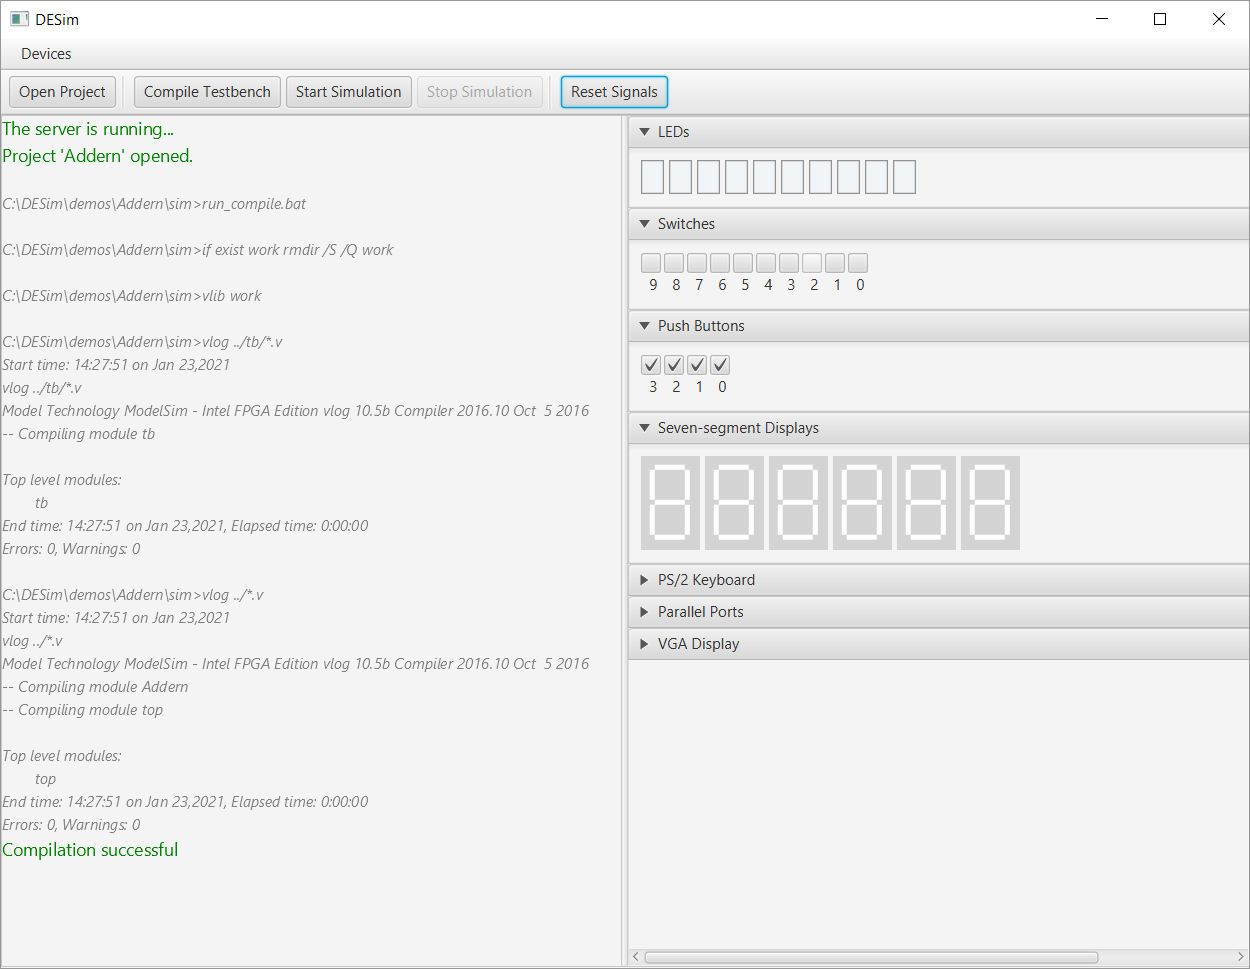
\includegraphics[width = \textwidth]{figures/run_compile.png}}
            \else
                \fbox{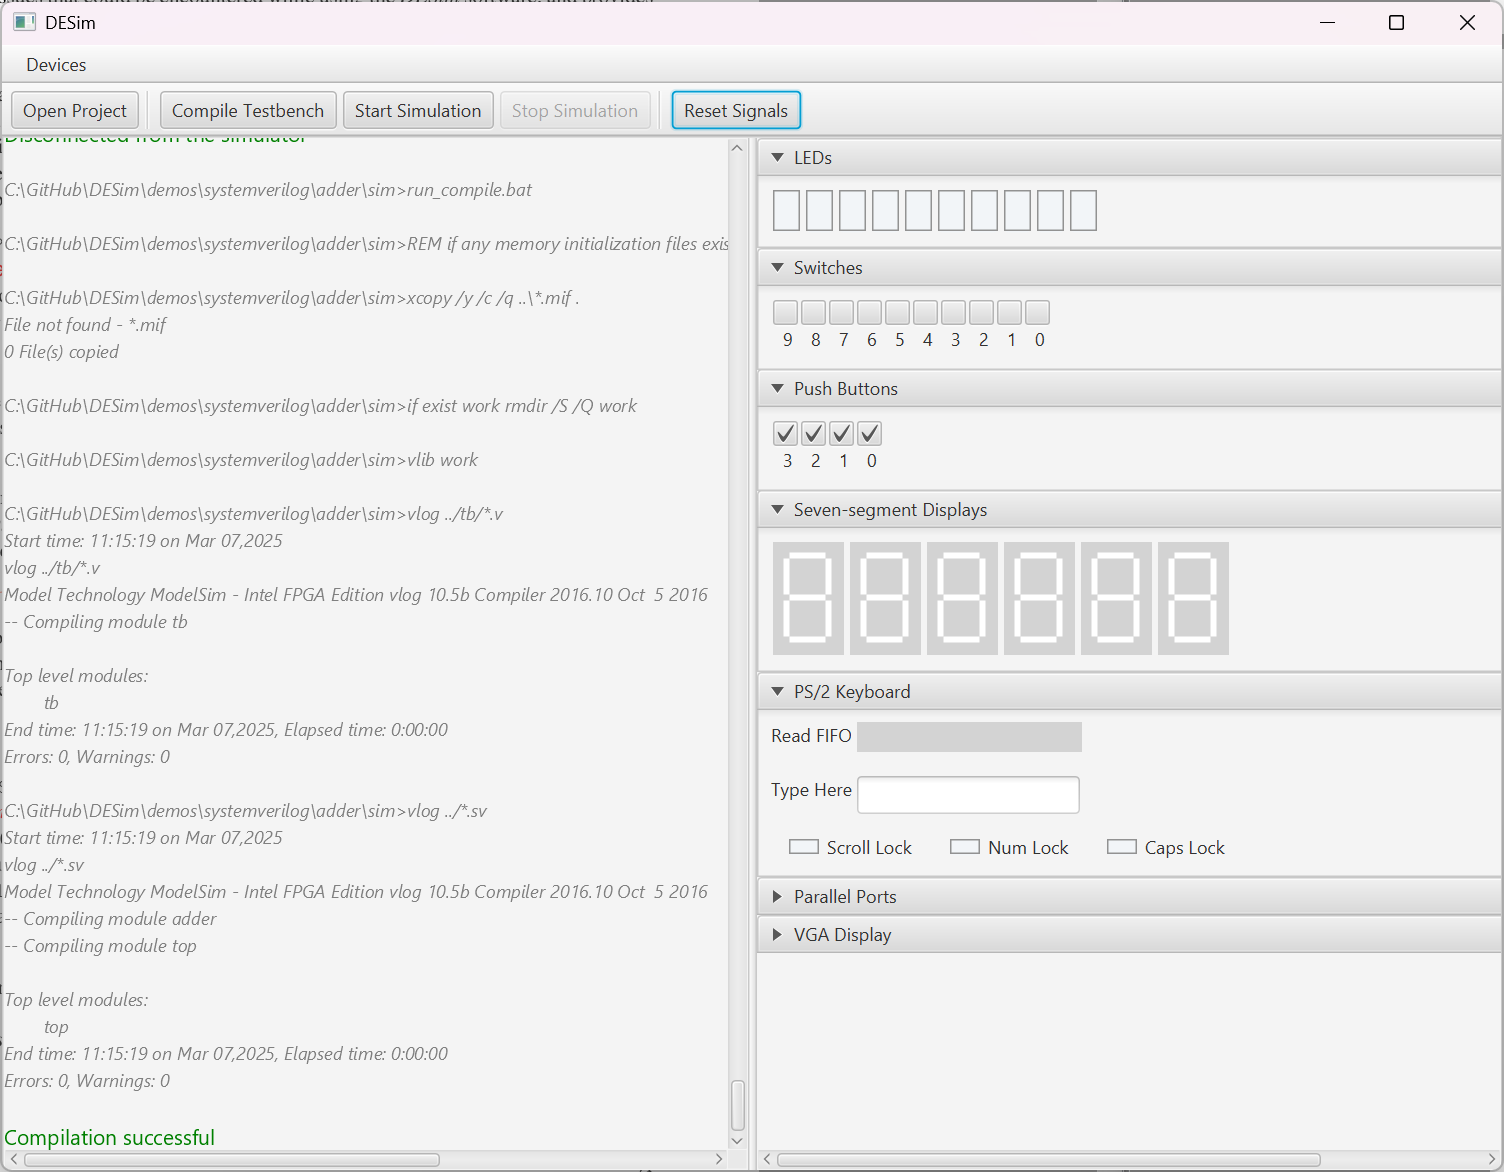
\includegraphics[width = .98\textwidth]{figures/run_compile_sv.png}}
            \fi
        \else
            \fbox{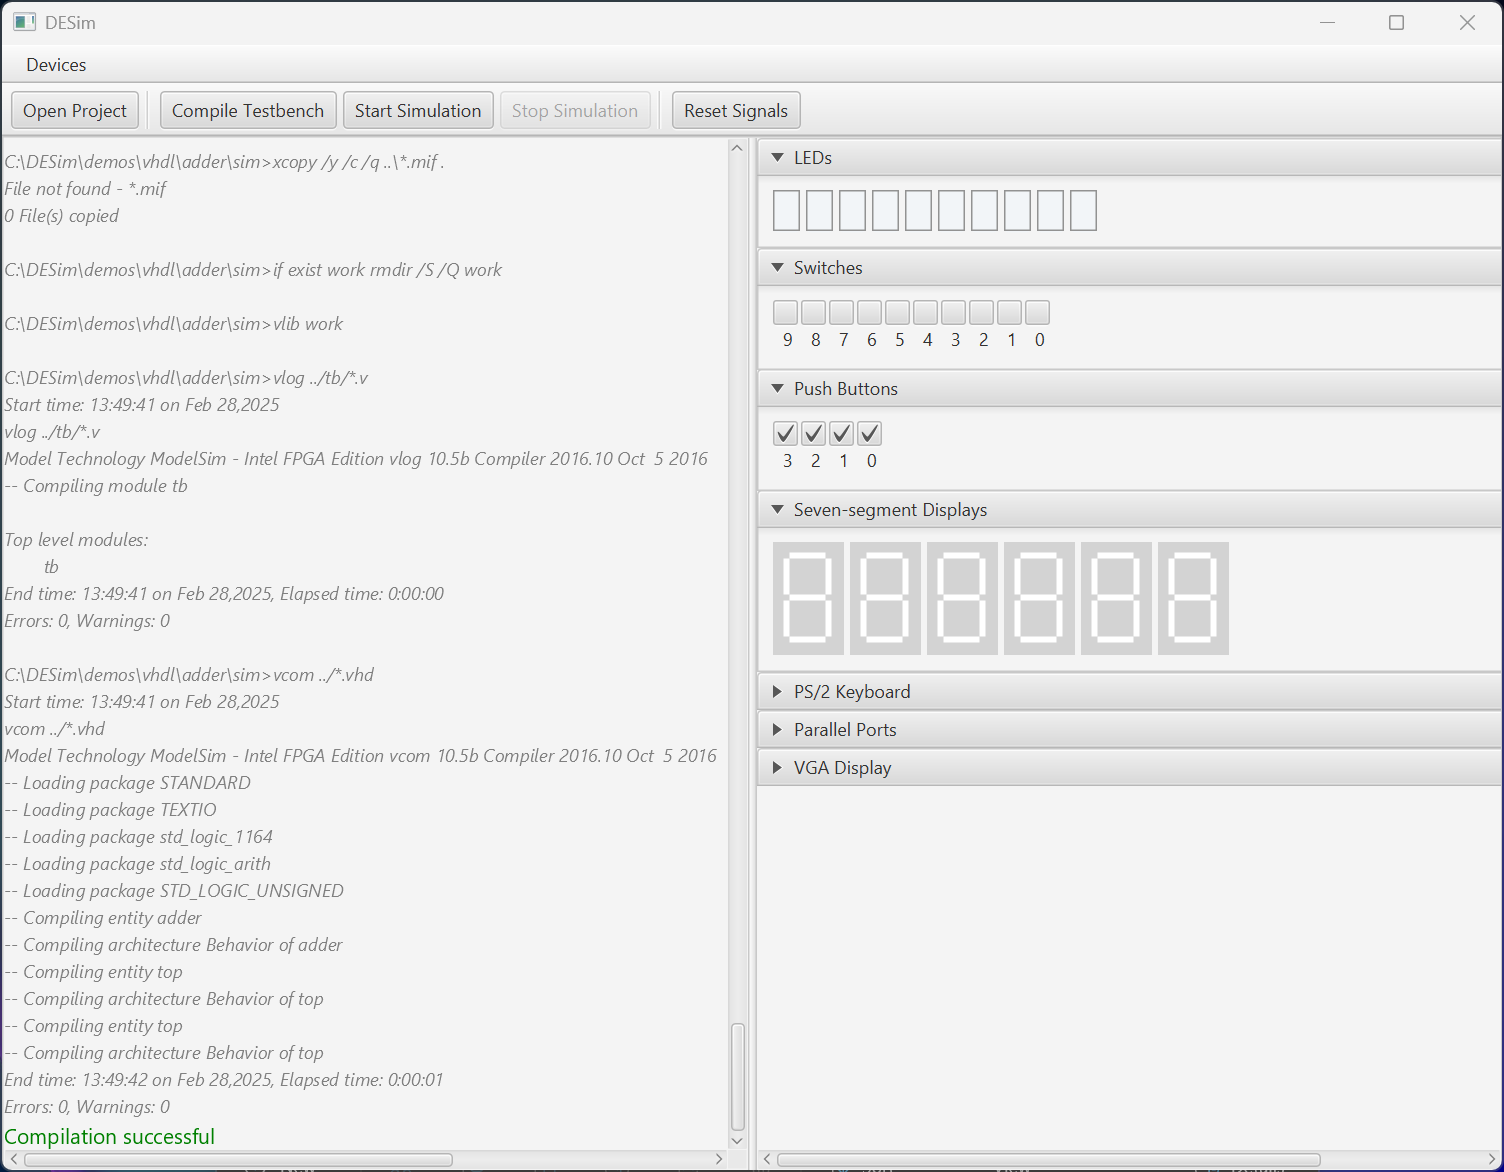
\includegraphics[width = \textwidth]{figures/run_compile_vhdl.png}}
        \fi
	\end{center}
          \caption{Messages produced by executing the {\it run\_compile} script.}
	\label{fig:compile}
\end{figure}

The testbench file for the {\it adder} project that is compiled by the command 
\texttt{vlog ../tb/*.v} is called {\it tb.v}, and is displayed in Figure~\ref{fig:tb}. 
It is not necessary to modify (or even examine) much of this code to use the {\it DESim}
application, but we describe some of the code here for completeness.  The testbench code 
has a general structure that allows it to be used to simulate different HDL code that might 
be used in various {\it DESim} projects. Hence, not all of the code in the testbench is 
needed for a particular project, such as our {\it adder} example. The first several lines in 
the {\it tb} \hdlModuleName~declare various signals that are used in the testbench. 

\begin{figure}[H]
\begin{center}
\begin{minipage}[t]{18 cm}
	\lstinputlisting[language=Verilog,numbers=none,linerange={9-47}]{../../demos/verilog/adder/tb/tb.v}
\end{minipage}
	\caption{The testbench file, {\it tb.v}, for the {\it adder} project.}
	\label{fig:tb}
\end{center}
\end{figure}

In Figure~\ref{fig:tb}, the statement

\lstinputlisting[language=Verilog,numbers=none,firstline=26,lastline=27]{../../demos/verilog/adder/tb/tb.v}

is unique to the {\it DESim} program. It makes use of a special feature of the
{\it ModelSim} (or {\it Questa}) software that allows communication with a 
{\it custom software function}. In this case, the custom function is part of the {\it DESim} 
software and is called {\it sim\_fpga}. This function is stored in a file named 
{\it modelsim.vpi} (or {\it questa.vpi}), which is located in the folder where {\it DESim} is
installed. The {\it DESim} GUI sends/receives signal values to/from the simulation software 
via the {\it sim\_fpga} function. 
This capability is known as the {\it Verilog Procedural Interface} (VPI). 

The statement

\lstinputlisting[language=Verilog,numbers=none,firstline=44,lastline=44]{../../demos/verilog/adder/tb/tb.v}

in the testbench code instantiates the {\it design under test} (DUT), which is the 
\hdlName~\hdlModuleName~named {\it top} shown in Figure~\ref{fig:top}. This instantiation
statement has to provide whatever port connections are needed for a particular {\it DESim}
project. Hence, if the project were using other/additional ports, then this
instantiation statement would need to be modified accordingly. Examples of different 
{\it top.\hdlFileExt}~files for other {\it DESim} projects are given later in this tutorial.

To execute the testbench using the simulator, click on the \texttt{Start Simulation} button 
in the {\it DESim} GUI. This command executes a script called {\it run\_sim}, which is found 
in the \texttt{sim} folder of the {\it adder} project. This script executes 
{\it vsim}, which is the {\it ModelSim} (or {\it Questa}) 
\hdlName~simulator, using the command

\ifverilog{\lstinputlisting[language=command.com]{../../demos/verilog/adder/sim/run_sim.bat}}
\else{\lstinputlisting[language=command.com]{../../demos/vhdl/adder/sim/run_sim.bat}}\fi

The \texttt{-pli} argument for the {\it vsim} program instructs 
it to link to the {\it sim\_fpga} custom software function that is provided in the
{\it modelsim.vpi} (or {\it questa.vpi}) file (the \texttt{DESimPath} and
\texttt{DESimulator} environment variables are set in the {\it DESim\_run.bat} script that is
used to start the {\it DESim} application, as discussed in Section \ref{sec:getting_started}).
The \texttt{-L} arguments include some simulation libraries for
Altera FPGAs that may be needed by the simulator. The \texttt{-t} argument specifies
the simulator time resolution. Finally, the remaining arguments 
run the simulation for the {\it tb} \hdlModuleName. Any messages 
produced while executing the {\it run\_sim} script are displayed inside the message pane in
the {\it DESim} GUI, as depicted in Figure~\ref{fig:sim}.

As mentioned previously, the {\it adder} project includes a {\it Readme.txt} file that
documents its usage. This file is displayed \ifverilog{in
Figure~\ref{fig:readme}}\else{below}\fi. You can follow
its instructions to see how the switches and lights are used for the project (of course, 
you can also garner this information by looking at the \hdlName~source code). An example
simulation result is illustrated in Figure~\ref{fig:sim}. It corresponds to {\it Cin} $= 1$,
$X = (0110)_2 = (6)_{10}$, and $Y = (1010)_2 = (10)_{10}$. The result of the addition,
$(10001)_2 = (17)_{10}$, is displayed on the \texttt{LEDs}. This result corresponds
to {\it Cout} $= 1$ and {\it S} $= (0001)_2$.  Try different settings for the
\texttt{SW} switches and observe the results displayed on the \texttt{LEDs}.

\begin{figure}[h]
	\begin{center}
        \setlength{\fboxsep}{0pt}
        \ifverilog
            \ifnotSV
                \fbox{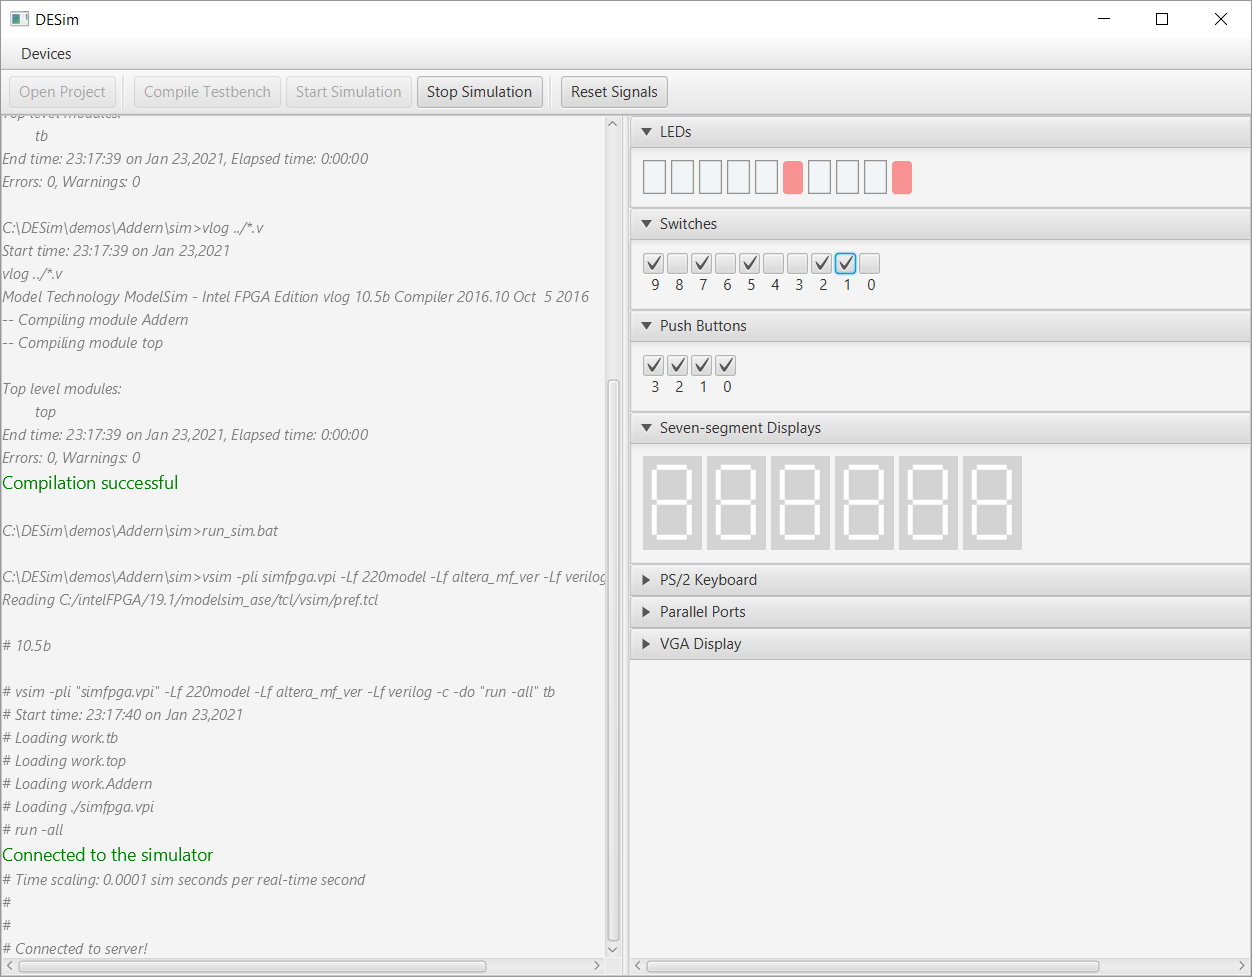
\includegraphics[width = \textwidth]{figures/run_simulation.png}}
            \else
                \fbox{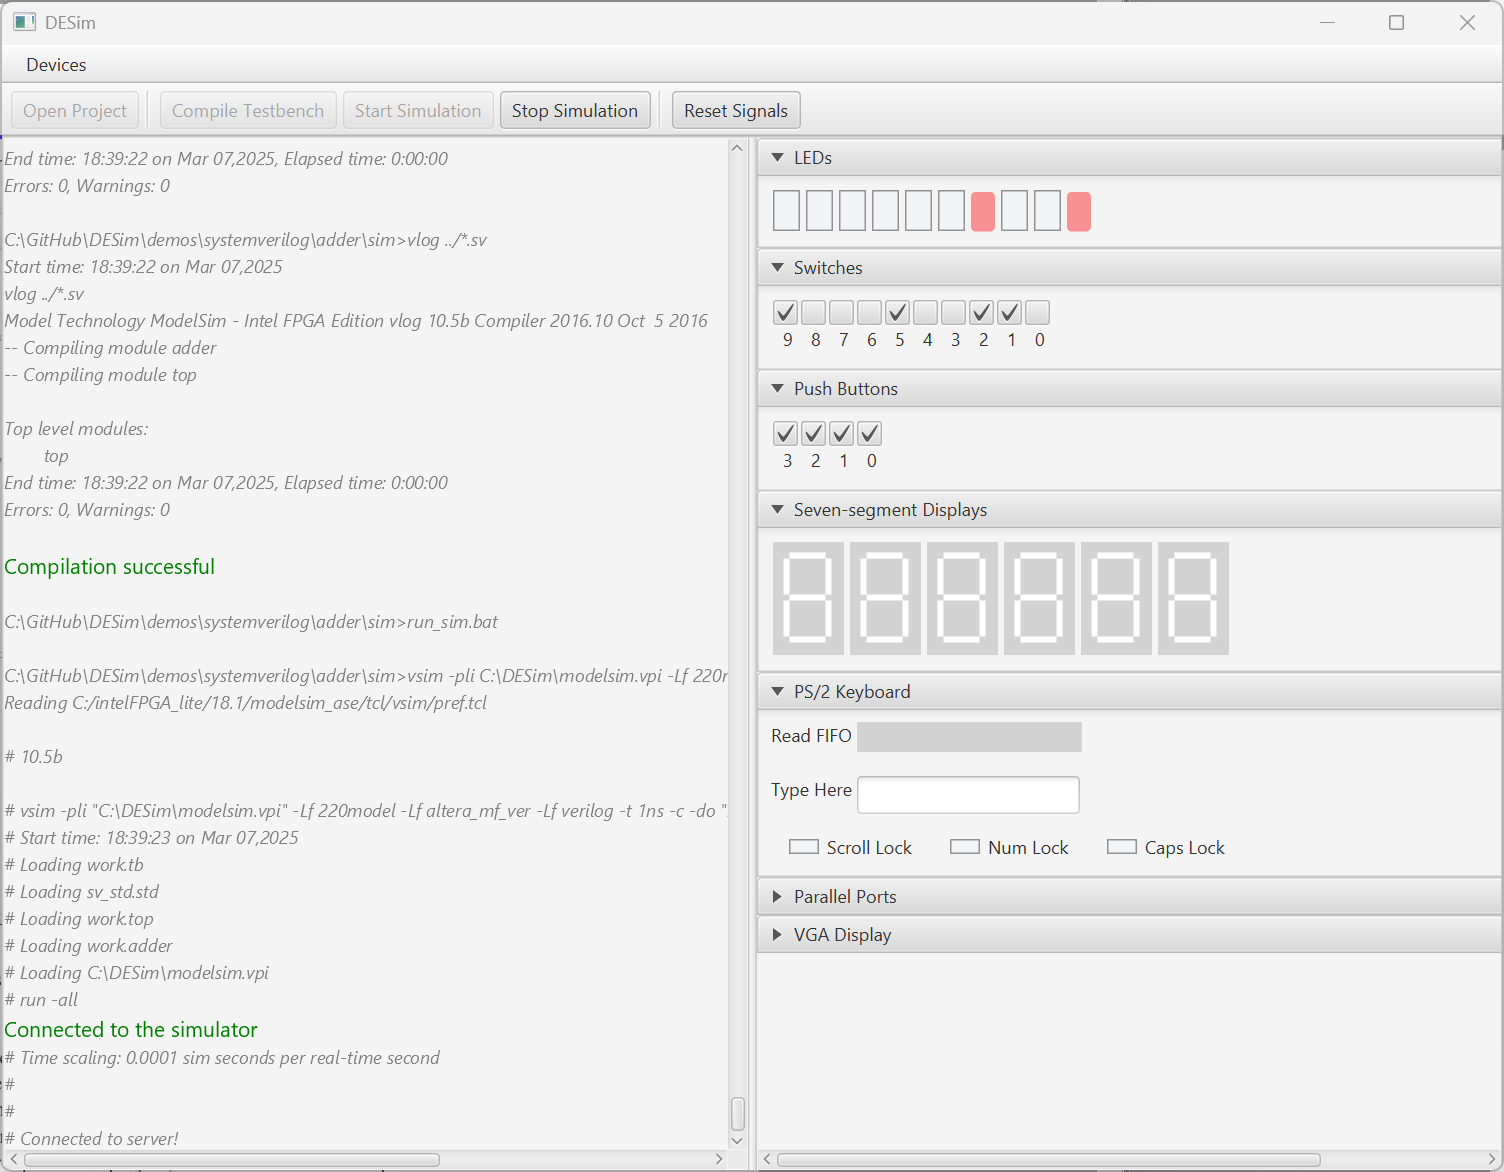
\includegraphics[width = \textwidth]{figures/run_simulation_sv.png}}
            \fi
        \else
            \fbox{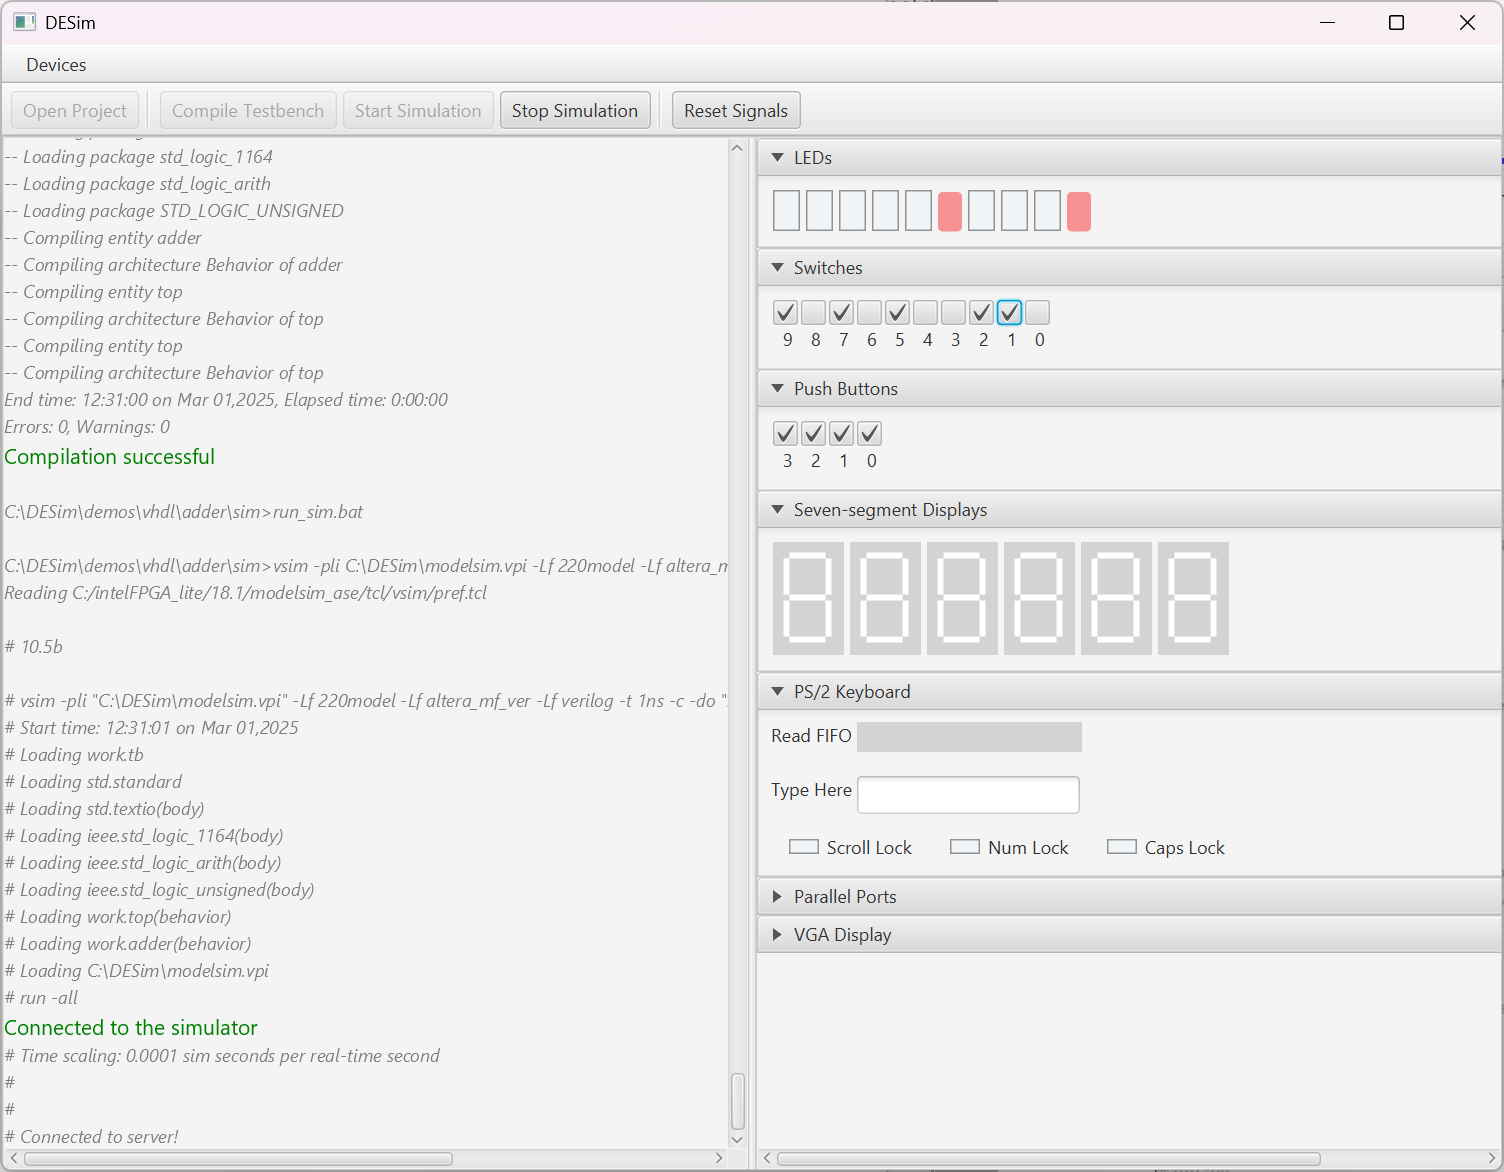
\includegraphics[width = \textwidth]{figures/run_simulation_vhdl.png}}
        \fi
	\end{center}
          \caption{Messages produced by executing the {\it run\_sim.} script.}
	\label{fig:sim}
\end{figure}

\ifverilog
\begin{figure}[H]
\begin{center}
    \begin{minipage}[t]{17 cm}
        \lstinputlisting[numbers=none]{../../demos/verilog/adder/Readme.txt}
    \end{minipage}
    \caption{The {\it Readme.txt} file for the {\it adder} project.}
	\label{fig:readme}
\end{center}
\end{figure}
\else
\begin{center}
\begin{minipage}[h]{17 cm}
    \lstinputlisting[numbers=none]{../../demos/vhdl/adder/Readme.txt}
\end{minipage}
\end{center}
\fi

\vspace{-0.25cm}
We have now finished discussing the {\it adder} sample project.

\section{Simulating a Sequential Circuit}

Another {\it DESim} sample project called {\it counter} is included in the {\it DESim}
\texttt{demos} folder. Use the \texttt{Open Project} button in the {\it DESim} GUI to open this
project. The contents of the filesystem folder for this project look the same as for the 
{\it adder} project, except that this project uses a \hdlName~source-code file named 
{\it counter.\hdlFileExt}.  Figure~\ref{fig:counter} shows the contents of 
the {\it counter.\hdlFileExt} file. It represents a 
24-bit counter with synchronous reset. The {\it LEDR} port name corresponds to the red LEDs
on a DE1-SoC board. Since {\it LEDR} port is a 10-bit signal and the 
counter has 24 bits, only a subset of the counter outputs (the most-significant ones) are 
connected to {\it LEDR}.

\begin{figure}[h]
\begin{center}
\begin{minipage}[h]{15 cm}
    \ifverilog
        \ifnotSV
            \lstinputlisting[language=Verilog,numbers=none,firstline=10]{../../demos/\demos/counter/Counter.\hdlFileExt}
        \else
            \lstinputlisting[language=Verilog,numbers=none,firstline=10, morekeywords={logic, always_ff}]{../../demos/\demos/counter/Counter.\hdlFileExt}
        \fi
    \else
        \lstinputlisting[language=VHDL,numbers=none,firstline=11]{../../demos/\demos/counter/Counter.vhd}
    \fi
\end{minipage}
	\caption{The \hdlName~code for the 24-bit counter.}
	\label{fig:counter}
\end{center}
\end{figure}

As described for the {\it adder} project, the {\it counter} \hdlModuleName~is {\it instantiated}
in another \hdlName~\hdlModuleName~called {\it top}. This \hdlModuleName~is displayed in 
Figure~\ref{fig:counter_top}. It is similar to the one from Figure~\ref{fig:top}, but it has
the appropriate ports ({\it CLOCK\_50}, {\it KEY}, and {\it LEDR}) needed for, and
instantiates, the {\it counter} \hdlModuleName.
As mentioned for the {\it adder} project, the port names for {\it top.\hdlFileExt}~correspond 
to signal names on the DE1-SoC board. 

\begin{figure}[h]
\begin{center}
\ifverilog
    \begin{minipage}[h]{15 cm}
        \ifnotSV
            \lstinputlisting[language=Verilog,numbers=none,firstline=7]{../../demos/\demos/counter/top.\hdlFileExt}
        \else
            \lstinputlisting[language=Verilog,numbers=none,firstline=7, morekeywords={logic, always_ff}]{../../demos/\demos/counter/top.\hdlFileExt}
        \fi
\else
    \begin{minipage}[h]{17 cm}
    \lstinputlisting[language=VHDL,numbers=none,firstline=8]{../../demos/\demos/counter/top.vhd}
\fi
\end{minipage}
	\caption{The {\it top} \hdlModuleName~for the {\it counter} project.}
	\label{fig:counter_top}
\end{center}
\end{figure}

To compile the {\it counter} project, in the {\it DESim} GUI click the \texttt{Compile Testbench}
button. It executes the {\it run\_compile} script, which
is found in the \texttt{sim} folder of the {\it counter} project. This script 
is identical to the one described earlier for the {\it adder} project. 
The testbench file that is compiled by {\it run\_compile} for the {\it counter} project is  
found in its \texttt{tb} folder. This testbench, {\it tb.v}, is the same as in
Figure~\ref{fig:tb}, except that it uses different ports in the instantiation statement
for the {\it top} \hdlModuleName, corresponding to those specified in 
Figure~\ref{fig:counter_top}.

To simulate the testbench for the {\it counter} project, click on the
\texttt{Start Simulation} button in the {\it DESim} GUI. This command executes the
{\it run\_sim} script. It is identical to that used for the 
{\it adder} project and runs the {\it vsim} simulator.

The {\it Readme.txt} file for the {\it counter} project, which describes its usage,
is shown in Figure~\ref{fig:readme_counter}. 

\begin{figure}[H]
\begin{center}
\begin{minipage}[t]{15 cm}
	\ifverilog
        \ifnotSV
            \lstinputlisting[numbers=none]{../../demos/verilog/counter/Readme.txt}
        \else
            \lstinputlisting[numbers=none]{../../demos/systemverilog/counter/Readme.txt}
        \fi
    \else
        \lstinputlisting[numbers=none]{../../demos/vhdl/counter/Readme.txt}
    \fi
\end{minipage}
    \caption{The {\it Readme.txt} file for the {\it counter} project.}
	\label{fig:readme_counter}
\end{center}
\end{figure}

\vspace{-0.5cm}
In the {\it DESim} GUI, when a \texttt{KEY} in the \texttt{Push Buttons} pane shows a check mark,
that {\it KEY} is set to the value 1. To reset the counter circuit, 
click on \texttt{KEY}$_0$ to {\it press} this button (this action sets the corresponding 
signal for this \texttt{KEY} to 0), and then click again to {\it release} the button. 
The 24-bit counter will start to operate and the ten
most-significant counter outputs will be displayed on the \texttt{LEDs}. A screen-shot of
the {\it DESim} GUI while simulating the {\it counter} project is illustrated in 
Figure~\ref{fig:sim2}.

\begin{figure}[h]
	\begin{center}
        \setlength{\fboxsep}{0pt}
        \ifverilog
            \ifnotSV
                \fbox{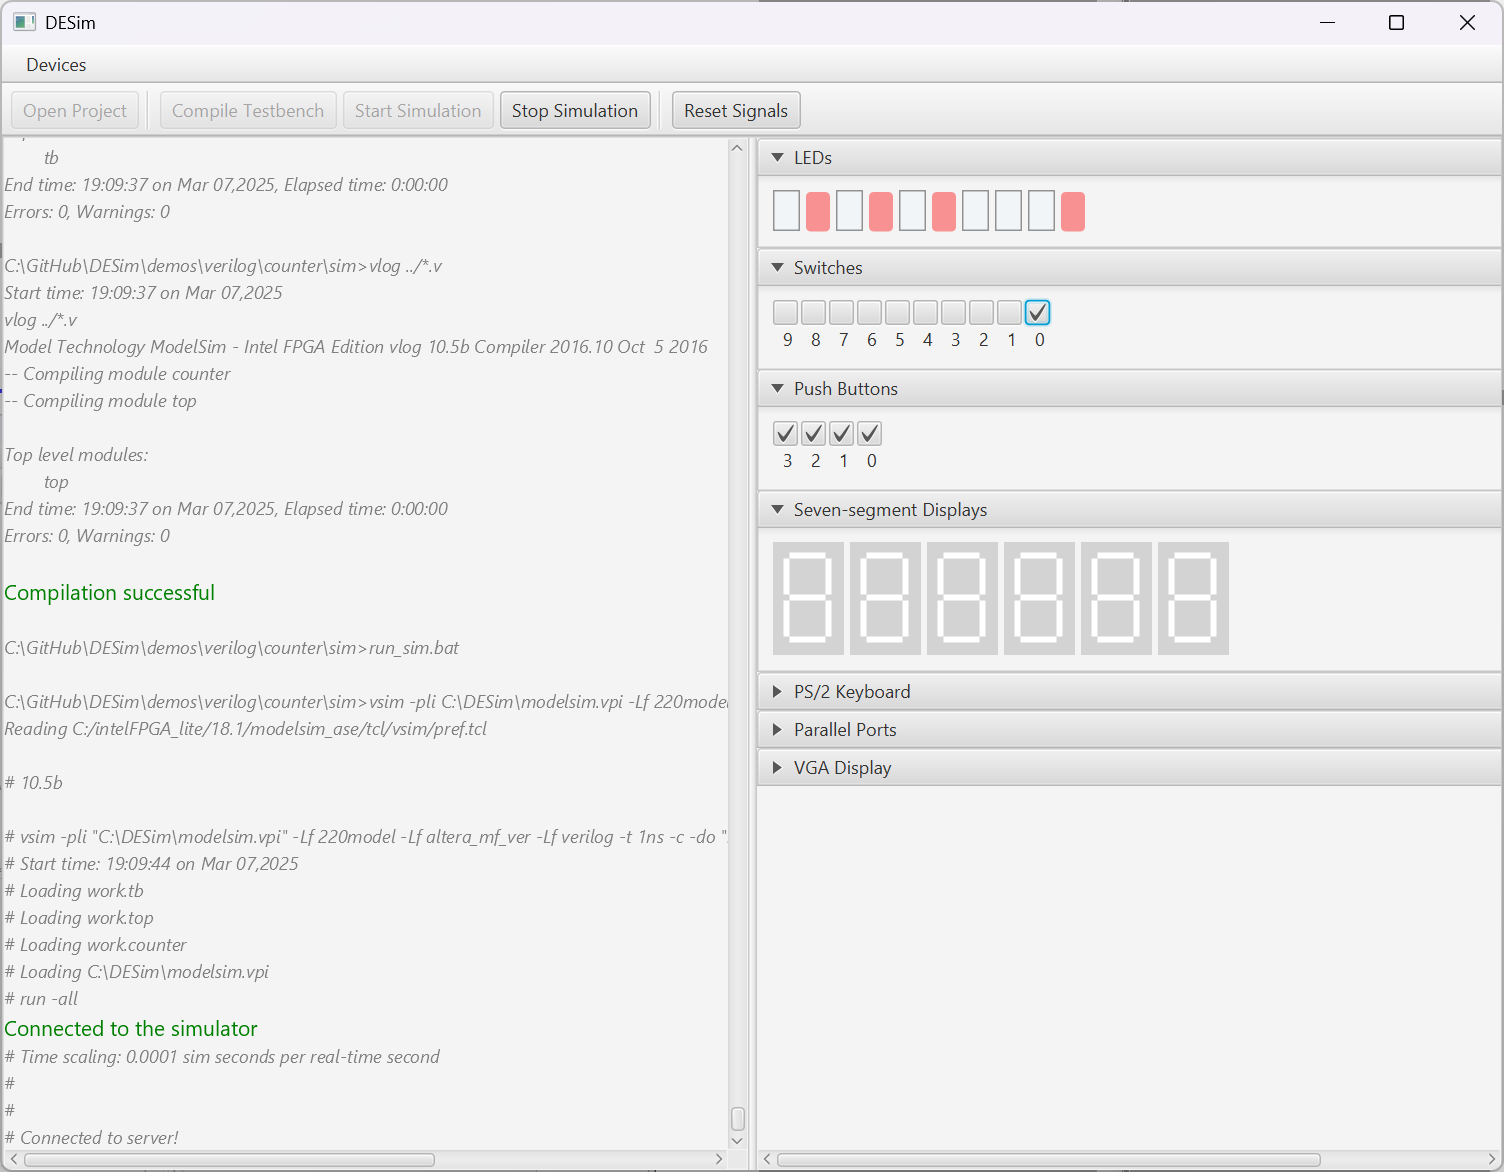
\includegraphics[width = \textwidth]{figures/run_simulation2.png}}
            \else
                \fbox{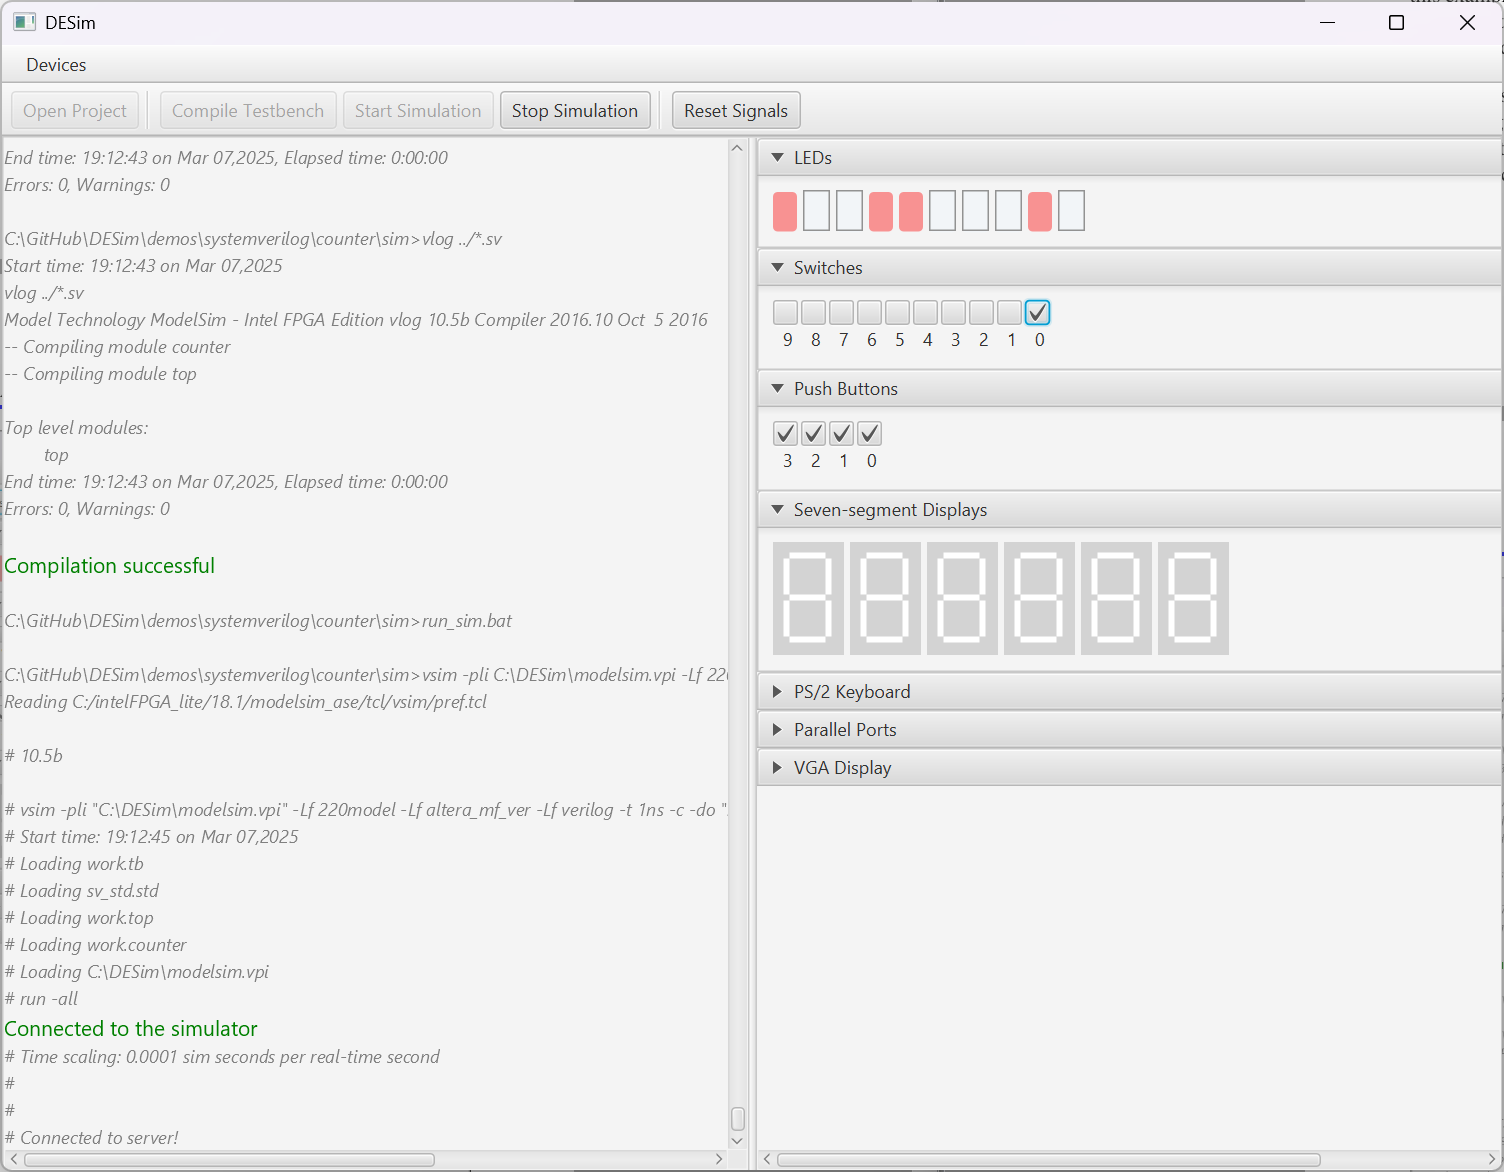
\includegraphics[width = \textwidth]{figures/run_simulation2_sv.png}}
            \fi
        \else
            \fbox{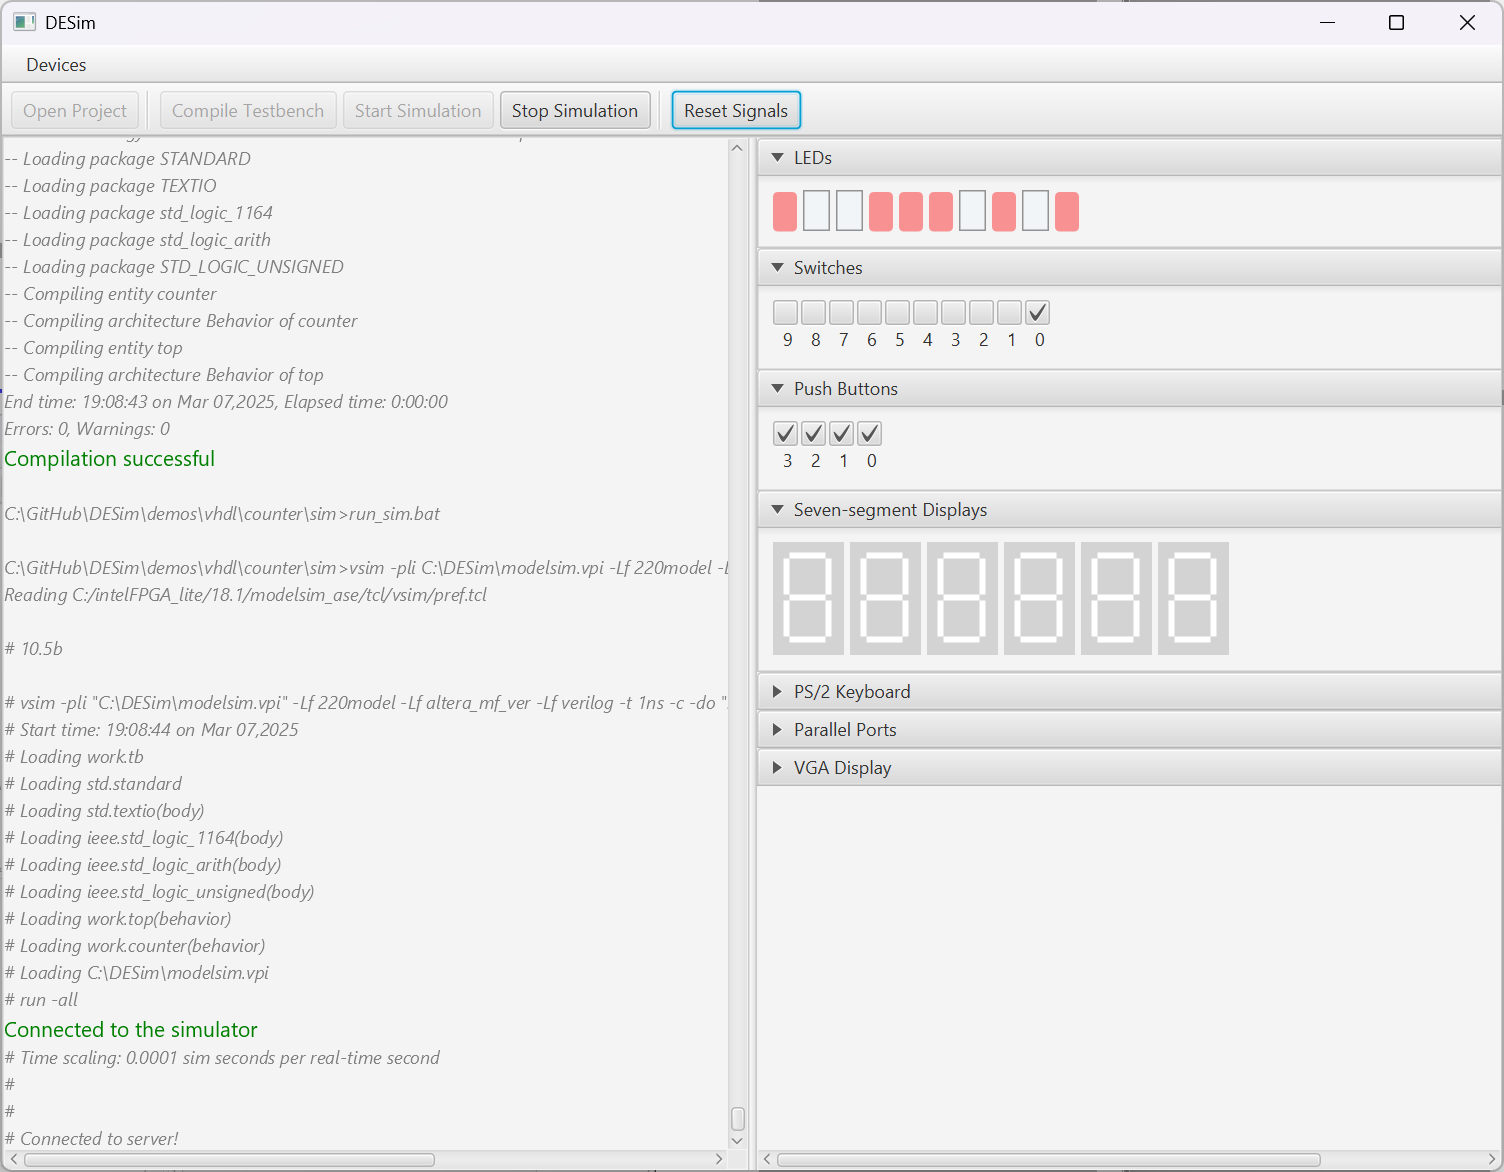
\includegraphics[width = \textwidth]{figures/run_simulation2_vhdl.png}}
        \fi
	\end{center}
          \caption{Simulating the {\it counter} project.}
	\label{fig:sim2}
\end{figure}

\section{Simulating a Circuit that Includes a Memory Module}

The {\it DESim} \texttt{demos} folder includes a project called {\it display}. It shows how 
to instantiate a memory module, and how to initialize the stored contents of 
this memory in a {\it DESim} simulation.  Use the \texttt{Open Project} command to open this
example project. The contents of the filesystem folder for this project look similar to the 
previous ones, but there are two extra files: {\it inst\_mem.v} and {\it inst\_mem.mif}. These 
files are used for the memory module in the circuit, which is described shortly.

Figure~\ref{fig:display} shows the \hdlName~code for {\it display.\hdlFileExt}, which 
has ports named {\it KEY}, {\it SW}, {\it HEX0}, and {\it LEDR}.
Figure~\ref{fig:memory}$a$ gives a logic circuit that corresponds to the code in 
Figure~\ref{fig:display}. The circuit contains a counter that is used to read the 
contents of successive locations in a memory. This memory provides codes in ASCII format 
for some upper- and lower-case letters, which are provided as inputs to a decoder \hdlModuleName. 
The counter and memory modules have a common clock signal, and the counter has a
synchronous clear input. Each successive clock cycle advances the counter and reads 
a new ASCII code from the memory. Since the counter is three-bits wide, only the first 
eight locations in the memory are read (the upper two address bits on the memory are set
to 00), and they provide the ASCII codes for letters A, b, C, d, E, F, g, and h. The 
decoder produces an appropriate bit-pattern to render each letter on a seven-segment display.
The ASCII code read from the memory is also displayed, on the LEDs.

The memory used in the logic circuit is depicted in part ($b$) of Figure~\ref{fig:memory}. It
is a $32 \times 8$ synchronous read-only memory (ROM), which has a register for holding 
address values. The memory is specified in the Verilog file {\it inst\_mem.v}, and it is 
initialized with the contents of the file {\it inst\_mem.mif},
which is illustrated in Figure~\ref{fig:mif}. This file contains the ASCII codes for the 
eight letters displayed by the circuit.

You may wish to examine the {\it top.\hdlFileExt} and {\it tb.v} files that are 
used for the {\it display} project.  These files are akin to those shown for the 
{\it adder} and {\it counter} projects, except that different ports are used for 
connecting to the {\it display} \hdlModuleName. 

\begin{figure}[h]
\begin{center}
\begin{minipage}[h]{15 cm}
\ifverilog
	\ifnotSV
        \lstinputlisting[language=Verilog,numbers=none,firstline=9]{../../demos/\demos/display/display.\hdlFileExt}
    \else
        \lstinputlisting[language=Verilog,numbers=none,firstline=9, morekeywords={logic, always_ff, always_comb}]{../../demos/\demos/display/display.\hdlFileExt}
    \fi
\else
	\lstinputlisting[language=VHDL,numbers=none,linerange={8-37}]{figures/display.vhd}
\fi
\end{minipage}
	\caption{The \hdlName~code for the {\it display} project\ifverilog{}\else{ (Part $a$)}\fi.}
	\label{fig:display}
\end{center}
\end{figure}

\ifverilog
{}
\else
    \begin{center}
    \begin{minipage}[h]{15 cm}
	    \lstinputlisting[language=VHDL,numbers=none,firstline=39]{figures/display.vhd}
    \end{minipage}
	    \center{The VHDL code for the {\it display} project (Part $b$).}
    \end{center}
\fi

\begin{figure}[t]
	\begin{center}
		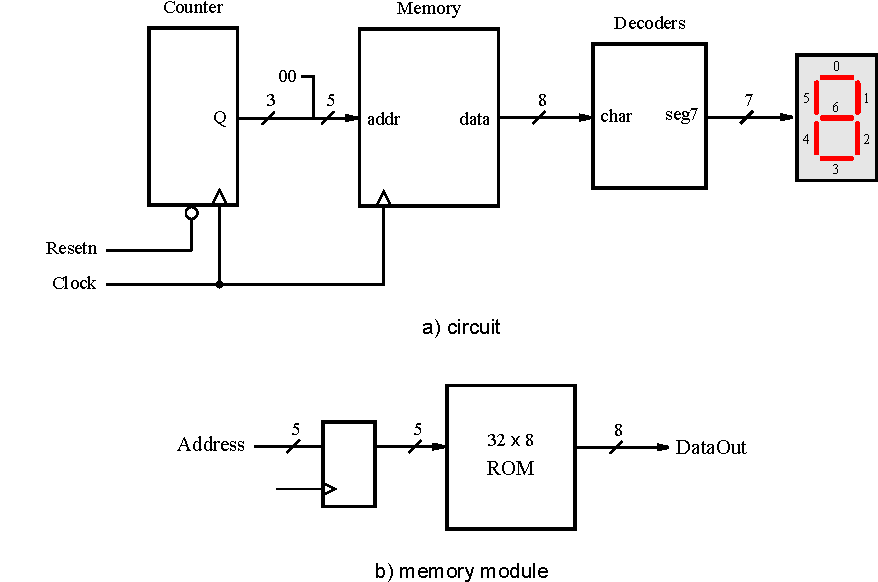
\includegraphics[scale = 1.0]{figures/figdisplay.pdf}
	\end{center}
          \caption{A circuit that represents the {\it display} project.}
	\label{fig:memory}
\end{figure}

\begin{figure}[bh!]
\begin{center}
\begin{minipage}[t]{12.5 cm}
\begin{tabbing}
DEPTH = 32;\\
WIDTH = 8;\\
ADDRESS\_RADIX = HEX;\\
DATA\_RADIX = DEC;\\
CONTENT\\
BEGIN\\
BEGI\=00X\=: \=104;XXXX\=\% A \=\% \kill
\>00 \>: \>65;    \>\% A \>\%\\
\>01 \>: \>98;    \>\% b \>\%\\
\>02 \>: \>67;    \>\% C \>\%\\
\>03 \>: \>100;   \>\% d \>\%\\
\>04 \>: \>69;    \>\% E \>\%\\
\>05 \>: \>70;    \>\% F \>\%\\
\>06 \>: \>103;   \>\% g \>\%\\
\>07 \>: \>104;   \>\% h \>\%\\
END;
\end{tabbing}
\end{minipage}
\end{center}
    \caption{The {\it inst\_mem.mif} memory initialization file.}
\label{fig:mif}
\end{figure}

\clearpage
\newpage
\noindent
To compile the {\it display} project, in the {\it DESim} GUI click the \texttt{Compile Testbench}
button. It executes, from the project's {\it sim} folder, the {\it run\_compile.bat} script
shown below: 

\lstinputlisting[language=command.com]{../../demos/\demos/display/sim/run_compile.bat}

The second line in the script copies the memory initialization file ({\it mif})
from the {\it display} project folder into the {\it sim}
folder. This is done for two reasons: {\it ModelSim} (or {\it Questa}) requires the file 
to be in the {\it sim} folder to properly initialize the memory module during a simulation, 
and copying the file from the {\it display} folder means that the latest version of the file 
will always be used for compilation and simulation. The rest of the script, which compiles the 
\ifverilog{Verilog }\else{VHDL }\fi code, is the same as for the previously-described 
{\it DESim} projects. To simulate the {\it display} project, click on 
the \texttt{Start Simulation} button.

The {\it Readme.txt} file for the {\it display} project is shown in Figure~\ref{fig:readme2}.
You can follow its instructions to read successive locations out of the memory and
display the corresponding characters on \red{HEX0}. An example simulation output after
first resetting the circuit and then creating a few clock cycles using {\it KEY}$_0$
is illustrated in Figure~\ref{fig:sim3}.

\lstset{language=make,escapechar=|}
\begin{figure}[h]
\begin{center}
\begin{minipage}[t]{15 cm}
	\lstinputlisting{../../demos/\demos/display/Readme.txt}
\end{minipage}
    \caption{The {\it Readme.txt} file for the {\it display} project.}
\label{fig:readme2}
\end{center}
\end{figure}

\begin{figure}[t]
	\begin{center}
        \setlength{\fboxsep}{0pt}
        \ifverilog
            \ifnotSV
                \fbox{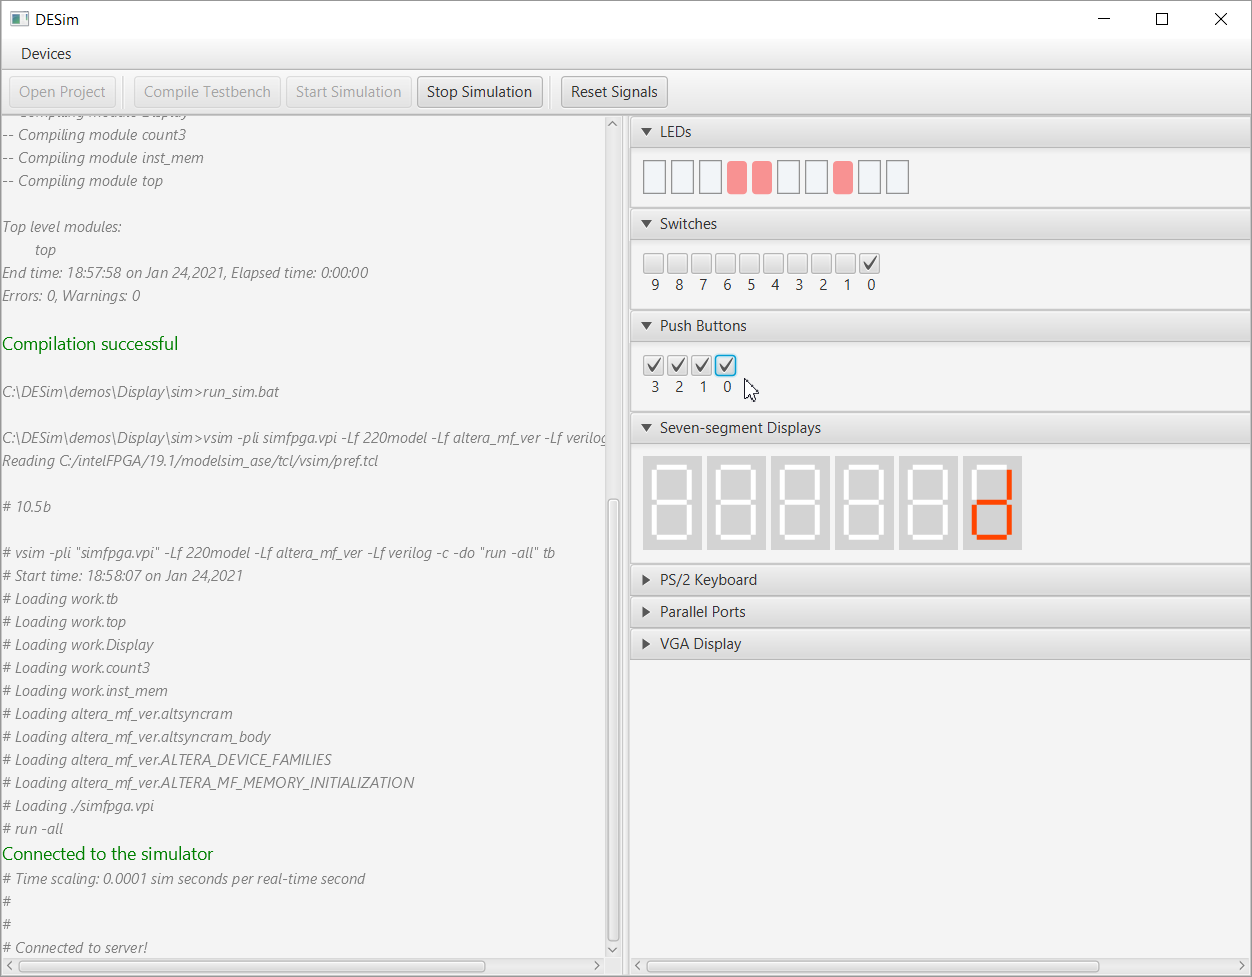
\includegraphics[width = \textwidth]{figures/run_simulation3.png}}
            \else
                \fbox{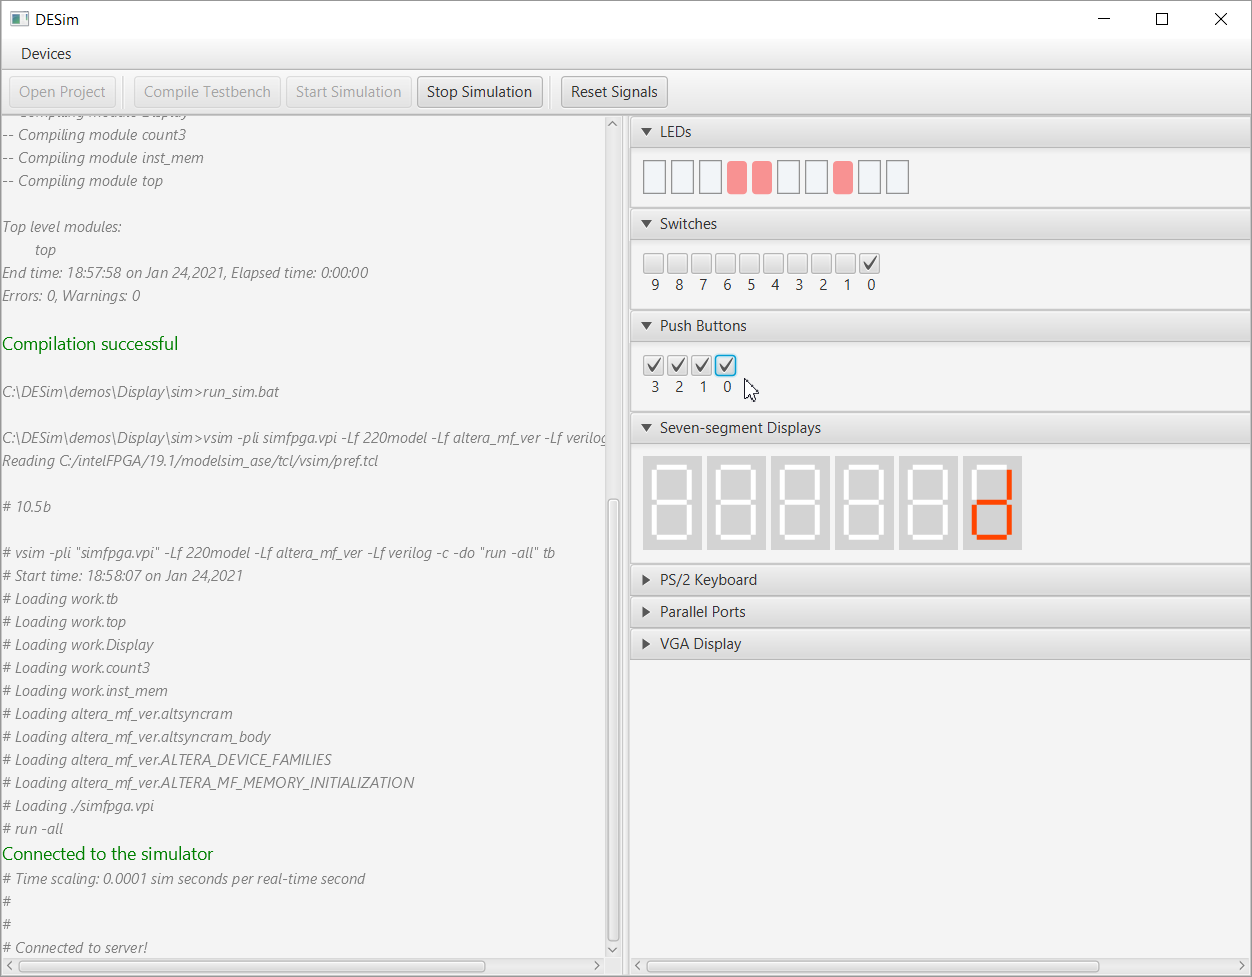
\includegraphics[width = \textwidth]{figures/run_simulation3.png}}
            \fi
        \else
            \fbox{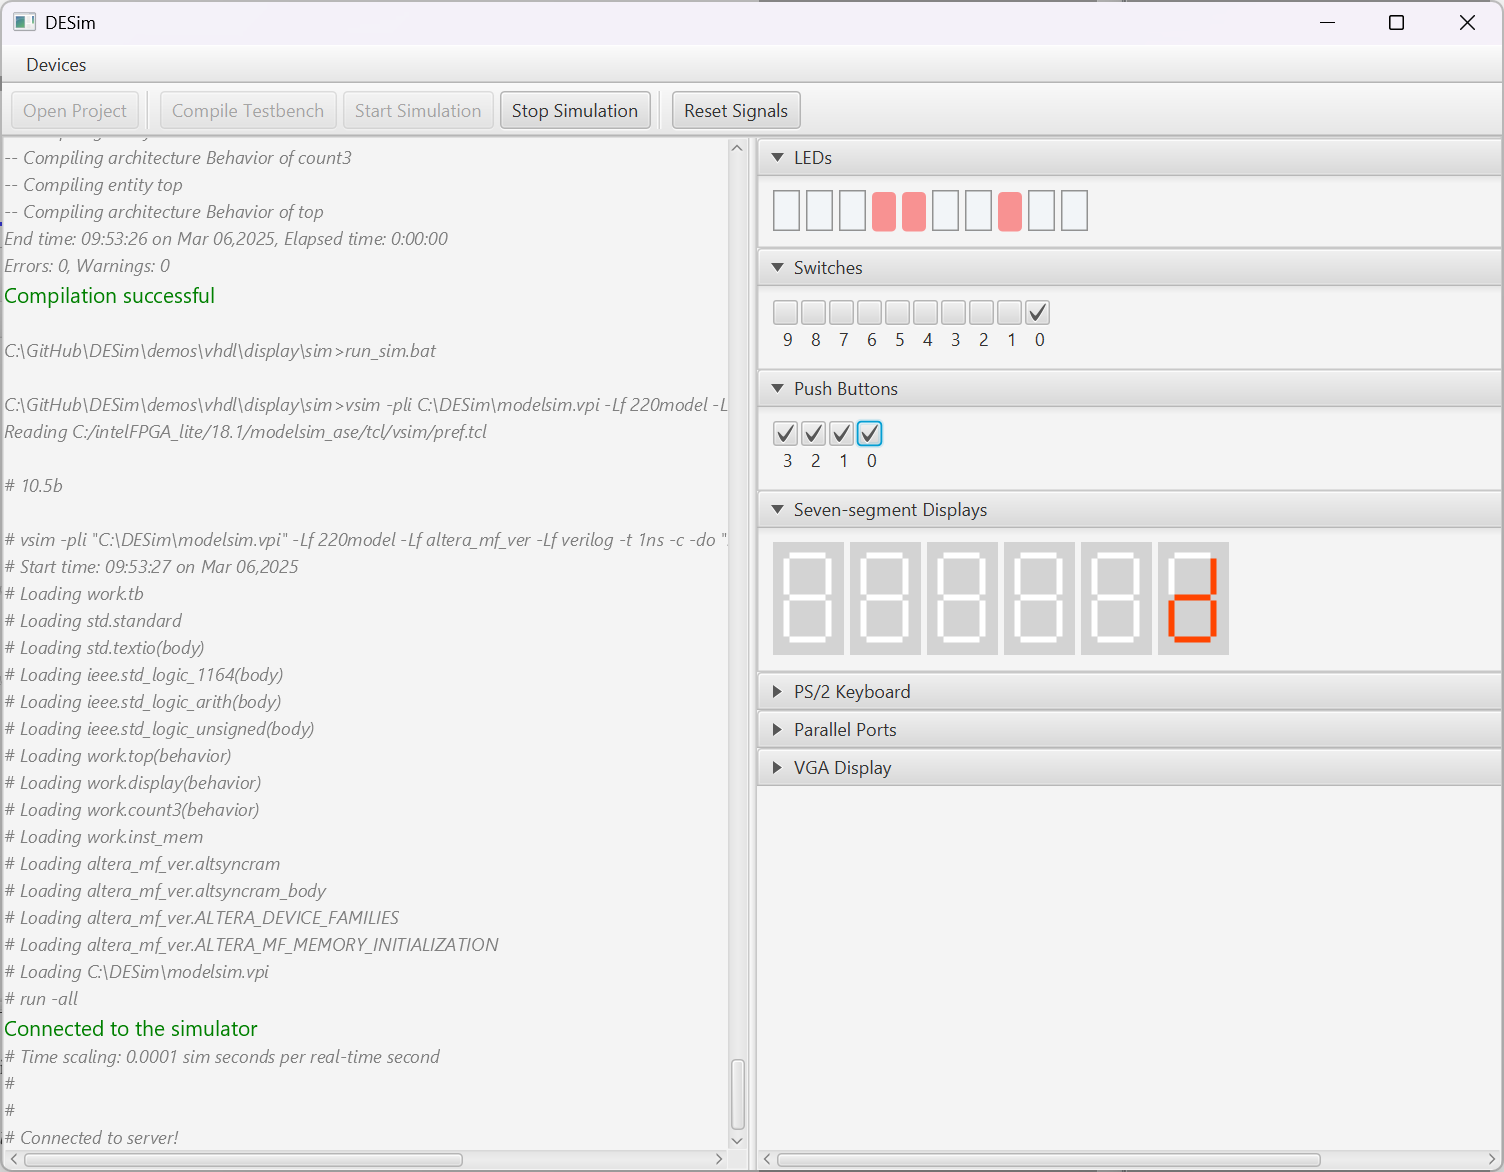
\includegraphics[width = \textwidth]{figures/run_simulation3_vhdl.png}}
        \fi
	\end{center}
          \caption{Simulating the {\it display} project.}
	\label{fig:sim3}
\end{figure}

\section{Setting Up Your Own {\it DESim} Project}

An easy way to set up your own {\it DESim} project is to use one of the sample projects in
the {\it DESim} \texttt{demos} folder as a starting point. You may want to choose 
a project that has similar ports to the ones that you need in its {\it top.\hdlFileExt }
\hdlModuleName~that is instantiated by its testbench. The various projects included in 
the \texttt{demos} folder may have different top-level ports. In general, once you make a
copy of one of the sample projects, you will only need to make sure that its
{\it top.\hdlFileExt } file has the ports that you need, and modify the code so that it
instantiates your new design. In the {\it tb} folder you will need 
to make corresponding changes to the statement in {\it tb.v } that instantiates your 
new {\it top} module.  You should not have to make any other modifications, either to the
testbench or to the files in the {\it sim} folder. 

\section{Advanced GUI Features}
\label{sec:advanced}
This section discusses three features of the {\it DESim} GUI that have not been used in the 
sample projects presented so far: \texttt{PS/2 Keyboard}, \texttt{Parallel Ports}, and 
\texttt{VGA Display}.

\subsection{PS/2 Keyboard}

The {\it DESim} \texttt{demos} folder includes a project called {\it ps2\_demo}. It shows how 
{\it DESim} allows you to include a PS/2 keyboard in your project.  The main design file in 
this project is named 
{\it ps2\_demo.\hdlFileExt }. It defines \ifverilog{a module }\else{an entity }\fi
called {\it ps2\_demo}, which has the ports:

\vspace{-0.5cm}
\begin{center}
\begin{minipage}[h]{15 cm}
\ifverilog
    \ifnotSV
        \lstinputlisting[language=Verilog,numbers=none,linerange={10-10}]{../../demos/\demos/ps2_demo/ps2_demo.\hdlFileExt}
    \else
        \lstinputlisting[language=Verilog,numbers=none,linerange={10-10}]{../../demos/\demos/ps2_demo/ps2_demo.\hdlFileExt}
    \fi
\else
	\lstinputlisting[language=VHDL,numbers=none,linerange={12-26}]{../../demos/\demos/ps2_demo/ps2_demo.vhd}
\fi
\end{minipage}
\end{center}

\vspace{-0.5cm}
These ports are similar to those used in other {\it DESim} projects, except for 
\texttt{ps2\_clk} and \texttt{ps2\_dat}. These ports represent the {\it PS/2 clock} and 
{\it PS/2 data} communications interface of an actual PS/2 keyboard. If you press a key on
such a keyboard, it generates waveforms on its {\it ps2\_clk} and {\it ps2\_dat} signals to 
transmit a {\it scan code} that represents the pressed key. In the {\it ps2\_demo} project 
the \texttt{ps2\_clk} and \texttt{ps2\_dat} signals are generated by a combination of the
{\it DESim} GUI and the testbench used in this sample project. This testbench
includes a Verilog module named {\it PS2\_Keyboard}. It processes the {\it scan codes}
generated by the {\it DESim} GUI and produces corresponding {\it serial} data using the
\texttt{ps2\_clk} and \texttt{ps2\_dat} signals. This serial data is the same as what
would be received from an actual PS/2 keyboard.

Use the \texttt{Open Project} button to open this sample project. As indicated in 
Figure~\ref{fig:ps2}, compile the project and then start the simulation. Make sure that
the contents of the \texttt{PS/2 Keyboard} pane are visible in the {\it DESim} GUI, as 
displayed in the figure. Reset the circuit by pressing/releasing \texttt{KEY}$_0$.
You should see the value \red{0} displayed on all six \texttt{Seven-segment displays}. 
Now, click your mouse pointer in the
\texttt{Type Here} box within the \texttt{PS/2 Keyboard} pane.  Press the `\texttt{a}' key
on your computer keyboard. This action causes {\it scan codes} \texttt{1C F0 1C} to be 
displayed inside the \texttt{Read FIFO} box in the \texttt{PS/2 Keyboard} pane. The first
code \texttt{1C} represents the key that has been pressed, the second code \texttt{F0} indicates
that a key has been {\it released}, and the third code \texttt{1C} specifies which key has
been released. Although these scan codes are part of the PS/2 {\it specification}, you can
change the codes generated for each key if desired, by modifying the contents of a file
named {\it scancode.csv}. It can be found in the folder where the {\it DESim} application
is installed. 

The {\it testbench} for the {\it ps2\_demo} project generates corresponding serial data, using
the \texttt{ps2\_clk} and \texttt{ps2\_dat} signals, for each of the scan codes in the 
\texttt{Read FIFO} box. This serial data is stored into {\it shift registers} in the 
{\it ps2\_demo} \hdlModuleName. It then displays the scan codes on the 
\texttt{Seven-segment Displays} in the {\it DESim} GUI. Now, in the \texttt{Type Here} box 
enter the `\texttt{s}' key. You will see the scan codes
\texttt{1b F0 1b} in both the \texttt{Read FIFO} box and on the 
\texttt{Seven-segment displays}. This result is shown in Figure~\ref{fig:ps2}.
Also, the {\it ps2\_demo} \hdlModuleName~displays on the \texttt{LEDs} the last ten bits of 
serial data that it has received on the \texttt{ps2\_clk} and \texttt{ps2\_dat} interface. 
In Figure~\ref{fig:ps2} the serial data displayed on the
\texttt{LEDs} represents \texttt{1100011011}. It shows, from right to left, the eight data
bits of the scan code \texttt{1B} followed by an {\it odd parity} bit (1) and a {\it stop}
bit (1).

Unlike other {\it DESim} sample projects, {\it ps2\_demo} includes a separate folder, 
called {\it Simulator}. It can be used to directly simulate in {\it ModelSim} (or {\it Questa}) 
the {\it PS2\_Keyboard} module that is provided as part of the {\it ps2\_demo} 
testbench. Running such a simulation allows you to examine the timing of the 
\texttt{ps2\_clk} and \texttt{ps2\_dat} signals that are generated for a scan code, as
illustrated by the example in Figure~\ref{fig:ps2_clk_dat}. It shows the \texttt{ps2\_clk} 
and \texttt{ps2\_dat} waveforms generated from the scan code \texttt{1b}. In the figure,
the yellow cursor, which is coincident with a falling edge of {\it ps2\_clk},
is aligned with the {\it start} bit that precedes the serial data, and
then the eight data bits of the scan code are aligned to subsequent falling edges
of {\it ps2\_clk}. Finally, there is a {\it parity} bit (1) and a {\it stop} bit (1). 

\begin{figure}[t]
	\begin{center}
        \setlength{\fboxsep}{0pt}
        \ifverilog
            \ifnotSV
                \fbox{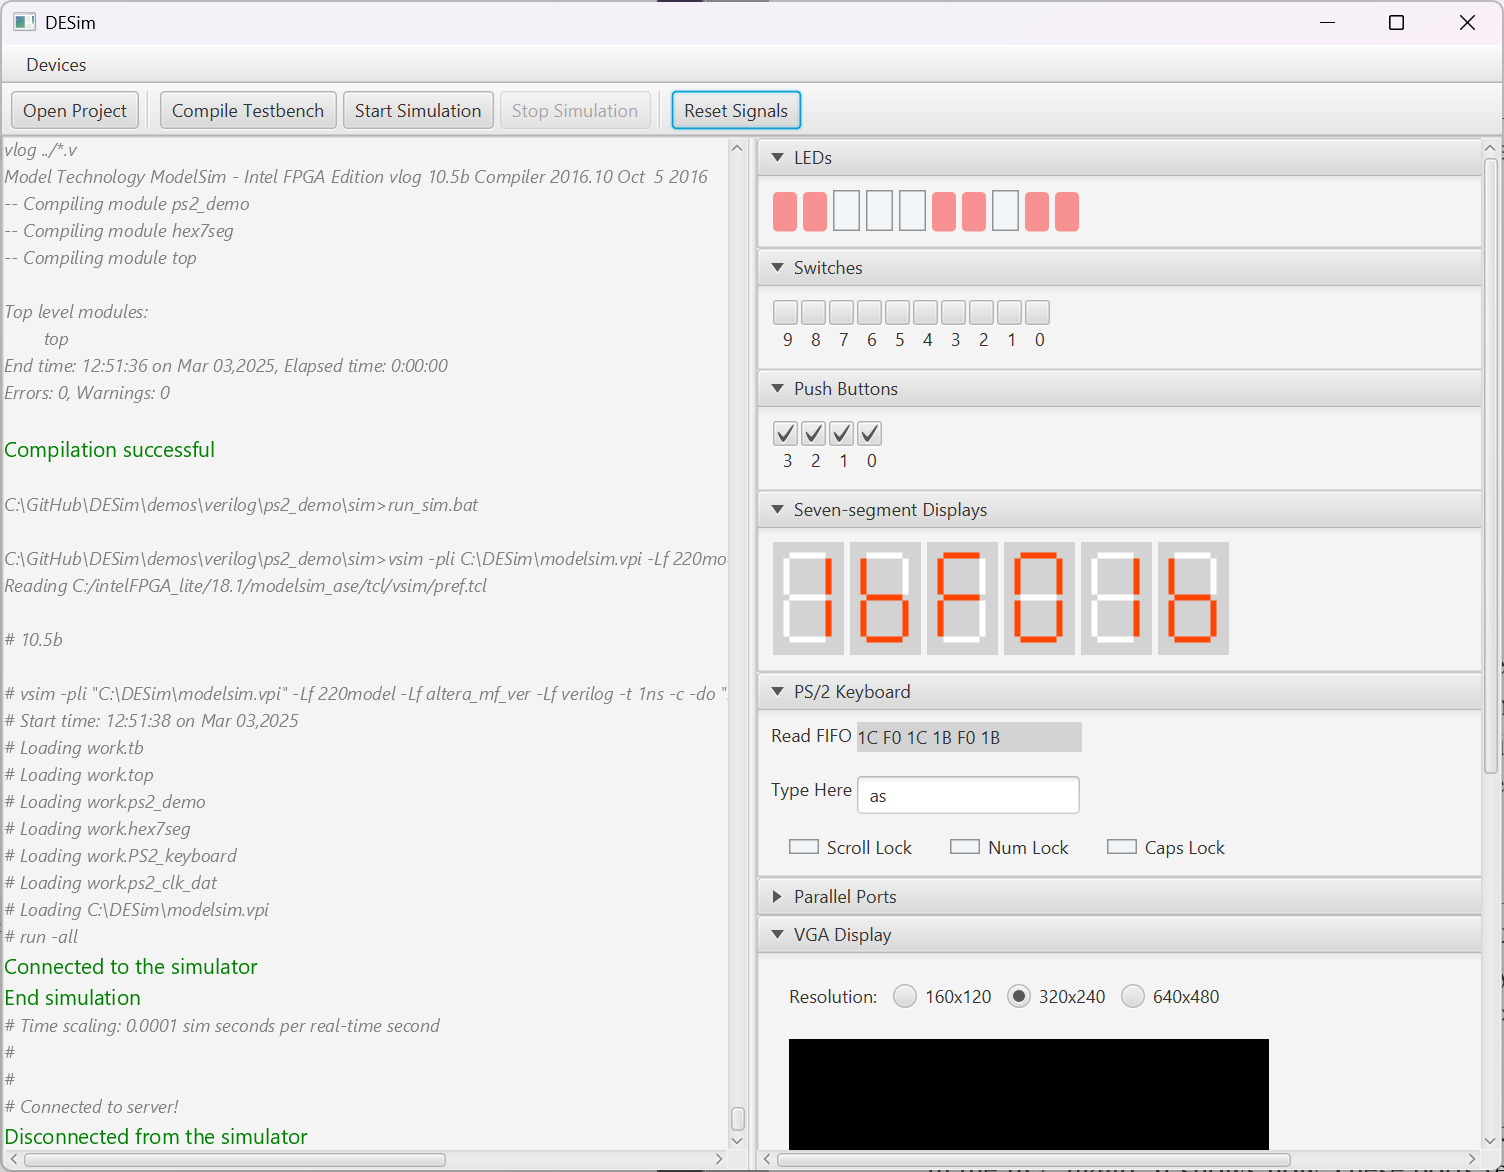
\includegraphics[width = \textwidth]{figures/ps2_demo.png}}
            \else
                \fbox{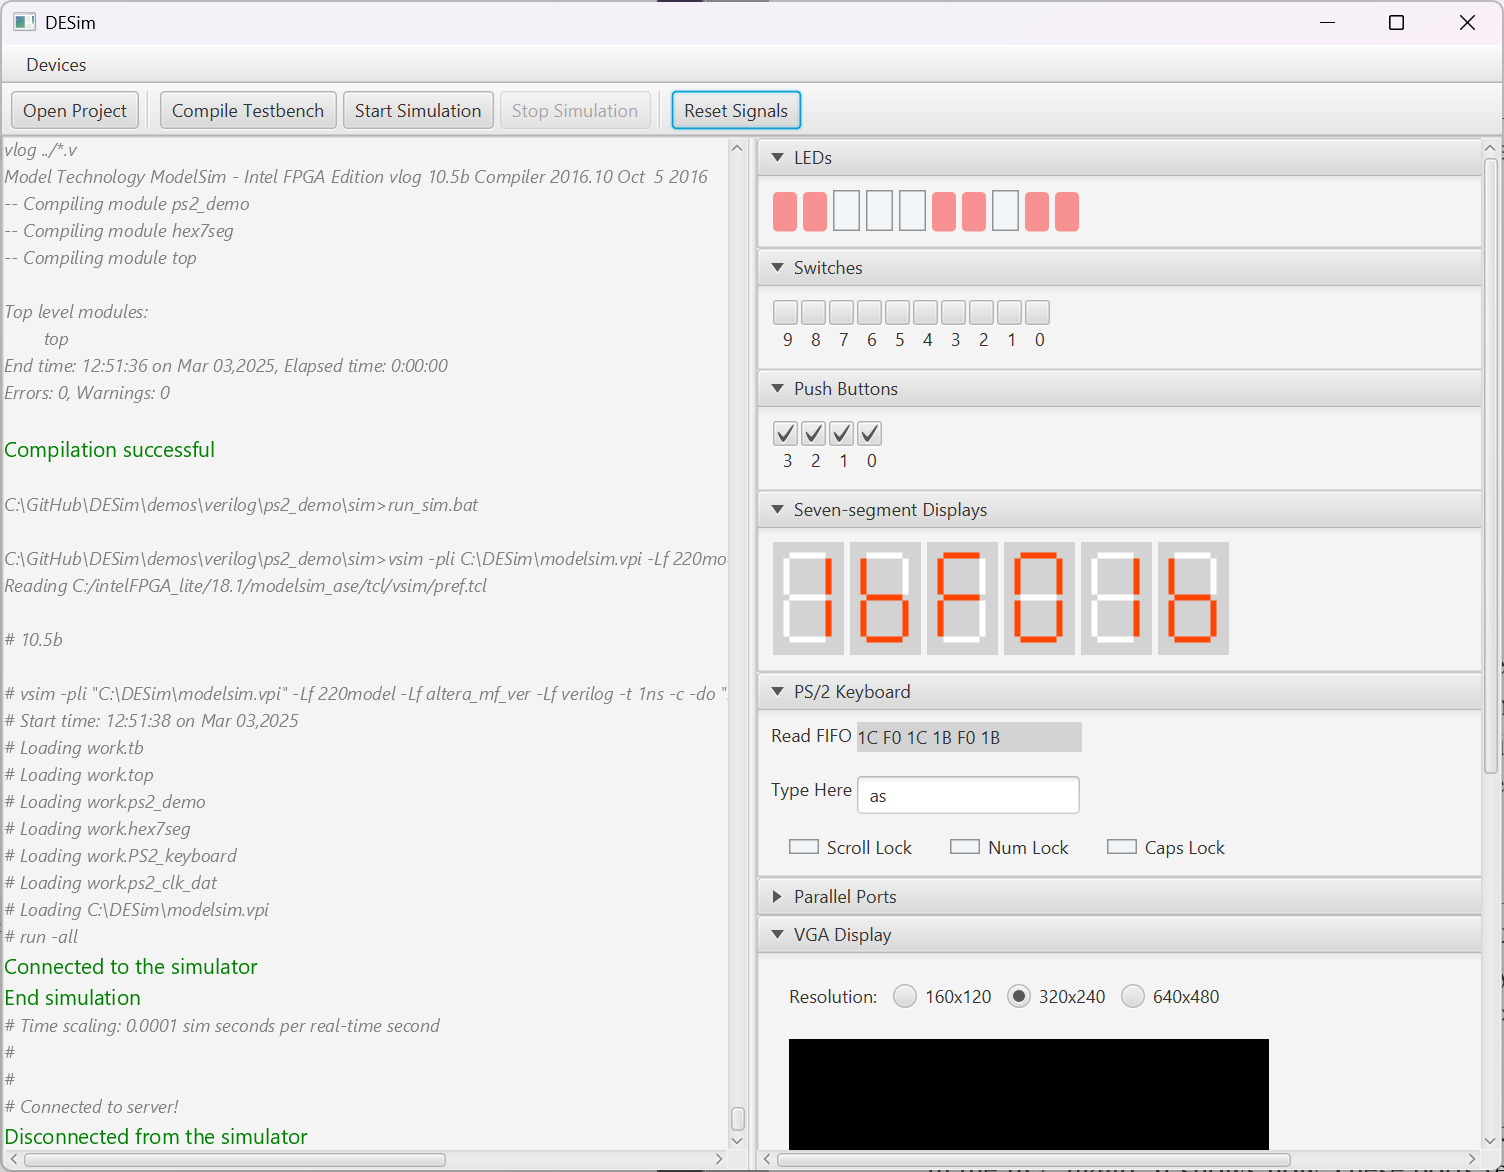
\includegraphics[width = \textwidth]{figures/ps2_demo.png}}
            \fi
        \else
            \fbox{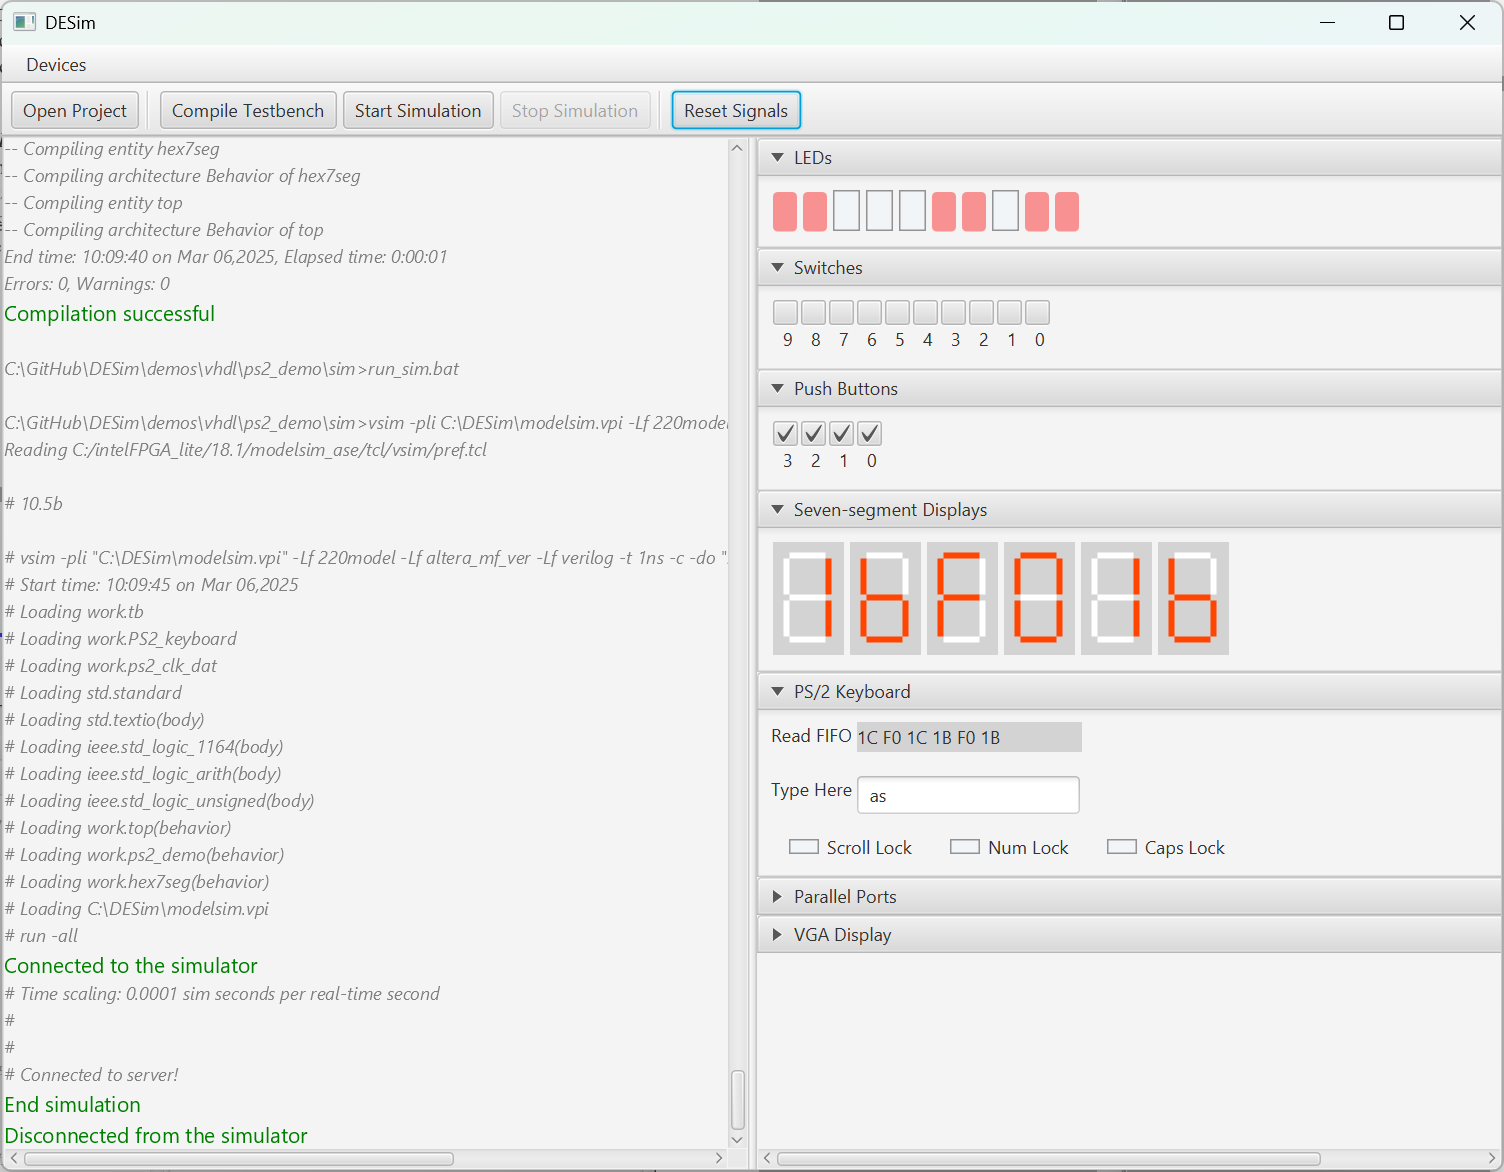
\includegraphics[width = \textwidth]{figures/ps2_demo_vhdl.png}}
        \fi
	\end{center}
          \caption{The {\it ps2\_demo} sample project.}
	\label{fig:ps2}
\end{figure}

\begin{figure}[h]
	\begin{center}
        \setlength{\fboxsep}{0pt}
        \fbox{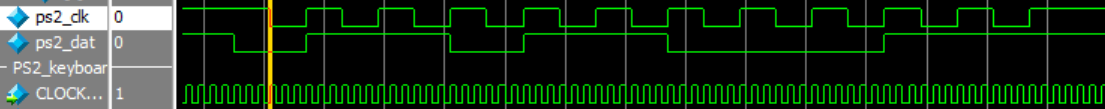
\includegraphics[width = .8\textwidth]{figures/ps2_clk_dat.png}}
	\end{center}
          \caption{PS/2 keyboard clock and data waveforms.}
	\label{fig:ps2_clk_dat}
\end{figure}

\subsection{Parallel Ports}

The {\it DESim} \texttt{demos} folder includes a project called {\it gpio}. It shows how 
the \texttt{Parallel Ports} pane in the {\it DESim} GUI can be used to represent the GPIO
expansion header on a DE1-SoC board. Open the {\it gpio} sample project, compile it, and
start the simulation in the {\it DESim} GUI. Figure~\ref{fig:gpio_pane} shows an example
of GPIO settings in the \texttt{Parallel Ports} while running the {\it gpio} demo. In the
figure, GPIO pins $15 - 0$ have their direction set as {\it inputs}, and pins $31 - 16$
are set as {\it outputs}. The {\it gpio} demo allows the input pins to be reflected on the
output pins in various ways. For Figure~\ref{fig:gpio_pane} the demo is set up to simply
reflect the values on GPIO pins $15 - 0$ onto pins $31 - 16$. Hence, in the top part of
the figure, pin 0 is reflected on pin 16, pin 1 or pin 17, and so on. You may wish to
examine the {\it Readme.txt} file for this sample project to see what other configurations
it supports.

\begin{figure}[h]
	\begin{center}
        \setlength{\fboxsep}{0pt}
        \fbox{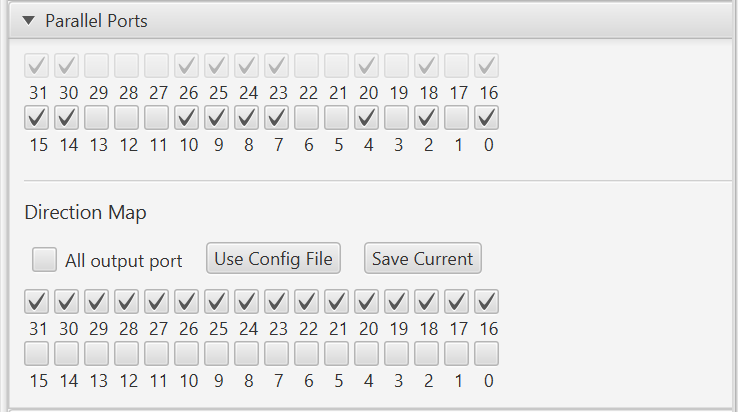
\includegraphics[width = .5\textwidth]{figures/gpio_pane.png}}
	\end{center}
          \caption{The \texttt{Parallel Ports} pane.}
	\label{fig:gpio_pane}
\end{figure}

\subsection{VGA Display}

The {\it DESim} \texttt{demos} folder includes a project called {\it vga\_demo}. It shows how 
you can use {\it DESim} to represent the VGA graphics video output on a DE1-SoC board.
The {\it top.\hdlFileExt}~\hdlModuleName~for this project is given in Figure~\ref{fig:vga}. It makes
connections to the {\it vga\_demo} \hdlModuleName~that allow addressing of pixels in a
emulated VGA ``screen''. Each of these pixels is located on a column and row of the 
``screen'' that is addressed using the \texttt{VGA\_X} port and \texttt{VGA\_Y} port,
respectively. A pixel's color is set using the \texttt{VGA\_COLOR} port, which allows for 
eight different {\it RGB} colors.  A pixel is plotted on the ``screen'' whenever the 
\texttt{plot} port is set to the value 1. Once a color is written into a pixel, it will
retain this color until it is changed again using the plot mechanism.

\begin{figure}[h]
\begin{center}
\begin{minipage}[h]{16 cm}
\ifverilog
    \ifnotSV
        \lstinputlisting[language=Verilog,numbers=none,firstline=1]{figures/top.\hdlFileExt}
    \else
        \lstinputlisting[language=Verilog,numbers=none,firstline=1, morekeywords={logic, always_ff, always_comb}]{figures/top.\hdlFileExt}
    \fi
\else
	\lstinputlisting[language=VHDL,numbers=none,firstline=8]{../../demos/\demos/vga_demo/top.\hdlFileExt}
\fi
\end{minipage}
	\caption{The {\it top.\hdlFileExt}~file for the {\it vga\_demo} project.}
	\label{fig:vga}
\end{center}
\end{figure}

Open the {\it vga\_demo} project, compile it, and then start the simulation. Make sure
that the \texttt{VGA Display} pane, depicted in Figure~\ref{fig:vga_pane}, is visible in
the {\it DESim} GUI. As shown in the figure, three ``screen'' resolutions are supported. 
Select the \texttt{320x240} resolution and then press/release {\it KEY}$_0$ to initialize 
the simulation. You should see the VGA ``screen'' filled with different colors, starting
with blue (color 001), then green (color 010), and so on. The image in the figure was
captured halfway through filling the ``screen'' with green. You may wish to examine the 
\hdlName~code in the file {\it vga\_demo.\hdlFileExt}~to learn more about how this sample
project works.

\begin{figure}[h]
	\begin{center}
        \setlength{\fboxsep}{0pt}
        \fbox{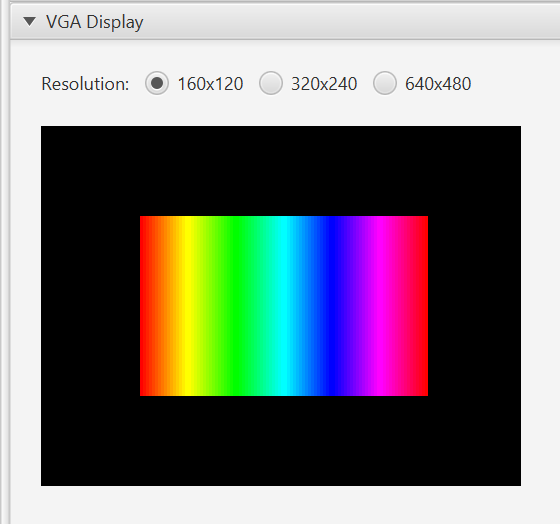
\includegraphics[width = .5\textwidth]{figures/vga_pane.png}}
	\end{center}
          \caption{The \texttt{VGA Display} pane.}
	\label{fig:vga_pane}
\end{figure}

\clearpage
\newpage
\section{Troubleshooting Problems with the {\it DESim} Software}
\label{sec:trouble}

This section discusses some potential issues that could be encountered while using the
{\it DESim} software, and provides suggested solutions.

\begin{enumerate}
\item Upon starting the {\it DESim} software you should see the message 
\green{The server is running...}'' at the top of the {\it message pane} in the GUI. If you do 
not see this message, but instead see a message \red{Server setup failed}, then 
the {\it DESim} software is not working properly and should be closed. One
reason why this would occur is if you have executed a {\it second}
instance of the {\it DESim} program. The {\it DESim} software cannot be
executed more than once concurrently on your computer. 

\item If you click on the \texttt{Compile Project} command in the {\it DESim} GUI, it is
possible to see an error message such as 
\red{`vlib' is not recognized as an internal or external command'}. This error means that
{\it DESim} attempted to execute the {\it vlib} program, which is part of the 
{\it ModelSim} (or {\it Questa}) software, but the program was not found by the
operating system. This error will occur if the {\it ModelSim} (or {\it Questa}) software 
is not installed on the computer, or if it is installed but cannot be be located. There are 
two ways to fix the latter issue: 1) the operating system \texttt{Path} environment variable 
can be updated to include the location of the {\it ModelSim} (or {\it Questa}) software, 
or 2) the location of the {\it ModelSim} (or {\it Questa}) software can be specified within 
the batch script that starts the {\it DESim} software. This script is called 
\texttt{DESim\_run.bat}, as described in Section~\ref{sec:getting_started}.

\item Occasionally, when compiling or simulating a project in the {\it DESim} software you may
see a {\it Warning} message which says that {\it ModelSim} (or {\it Questa}) cannot 
``unlink'' a file.  For example, if your {\it DESim} project is stored in the folder
C:$\backslash$DESim$\backslash$demos$\backslash$adder, then this message would report: 

\noindent
\begin{minipage}[h]{18 cm}
\lstset{language=command.com,numbers=none,escapechar=|,moredelim=**[is][\color{RedOrange}]{@}{@}}
\begin{lstlisting}[]
@** Warning: (vlog-31) Unable to unlink file "C:/DESim/demos/adder/sim/work/_lock"@
\end{lstlisting}
\end{minipage}

This problem occurs for unknown reasons and is not caused by the {\it DESim} application 
(it has also been observed when directly using the {\it ModelSim} (or {\it Questa}) Simulators
outside of the {\it DESim} environment). 
If the ``unlink'' issue persists (sometime it gets resolved 
automatically), then a solution is to browse with \texttt{File Explorer} into the filesystem
folder  
\texttt{C:$\backslash$DESim$\backslash$demos$\backslash$adder$\backslash$sim$\backslash$work}
and manually {\it delete} the file named {\it \_lock}.

\item When you click on the \texttt{Start Simulation} button in the {\it DESim} GUI,
you could see an error message such as \red{Load of {\it C:/DESim/modelsim.vpi}
(or {\it C:/DESim/questa.vpi}) failed: Bad DLL Format}.
This error occurs if you try to use the {\it ModelSim} (or {\it Questa}) Simulator with
the wrong {\it vpi} file.  The solution to this problem is to edit the batch file that is
used to start the {\it DESim} application, \texttt{DESim\_run.bat}, and ensure that the
environment variable \texttt{DESimulator} that is set in this script has the correct value
({\it modelsim} or {\it questa}), which matches the Simulator that you are using.

\item When you click on the \texttt{Start Simulation} button in the {\it DESim} GUI, it is
possible that the expected outputs in the {\it DESim} GUI will not be displayed. If this
occurs, then examine the {\it transcript} file that is stored in the project's {\it sim} folder. 
This {\it transcript} may provide insight by showing errors or warning that have been produced
by {\it ModelSim} (or {\it Questa}) due to issues with your HDL code.

\end{enumerate}

% Copyright and Trademark

\input{\commonPath/Docs/copyright.tex}

\end{document}
